%!TEX TS-program = xelatex
\documentclass[a4paper,14pt]{article}


%%% Работа с русским языком
\usepackage[english,russian]{babel}   %% загружает пакет многоязыковой вёрстки
\usepackage{fontspec}      %% подготавливает загрузку шрифтов Open Type, True Type и др.
\defaultfontfeatures{Ligatures={TeX},Renderer=Basic}  %% свойства шрифтов по умолчанию
\setmainfont[Ligatures={TeX,Historic}]{Times New Roman} %% задаёт основной шрифт документа
\setsansfont{Comic Sans MS}                    %% задаёт шрифт без засечек
\setmonofont{Courier New}
\usepackage{indentfirst}
\frenchspacing

\renewcommand{\epsilon}{\ensuremath{\varepsilon}}
\renewcommand{\phi}{\ensuremath{\varphi}}
\renewcommand{\kappa}{\ensuremath{\varkappa}}
\renewcommand{\le}{\ensuremath{\leqslant}}
\renewcommand{\leq}{\ensuremath{\leqslant}}
\renewcommand{\ge}{\ensuremath{\geqslant}}
\renewcommand{\geq}{\ensuremath{\geqslant}}
\renewcommand{\emptyset}{\varnothing}

%%% Дополнительная работа с математикой
\usepackage{amsmath,amsfonts,amssymb,amsthm,mathtools} % AMS
\usepackage{icomma} % "Умная" запятая: $0,2$ --- число, $0, 2$ --- перечисление

%% Номера формул
%\mathtoolsset{showonlyrefs=true} % Показывать номера только у тех формул, на которые есть \eqref{} в тексте.
%\usepackage{leqno} % Нумерация формул слева	

%% Перенос знаков в формулах (по Львовскому)
\newcommand*{\hm}[1]{#1\nobreak\discretionary{}
	{\hbox{$\mathsurround=0pt #1$}}{}}

%%% Работа с картинками
\usepackage{graphicx}  % Для вставки рисунков
\graphicspath{{images/}}  % папки с картинками
\setlength\fboxsep{3pt} % Отступ рамки \fbox{} от рисунка
\setlength\fboxrule{1pt} % Толщина линий рамки \fbox{}
\usepackage{wrapfig} % Обтекание рисунков текстом

%%% Работа с таблицами
\usepackage{array,tabularx,tabulary,booktabs} % Дополнительная работа с таблицами
\usepackage{longtable}  % Длинные таблицы
\usepackage{multirow} % Слияние строк в таблице
\usepackage{float}% http://ctan.org/pkg/float

%%% Программирование
\usepackage{etoolbox} % логические операторы


%%% Страница
\usepackage{extsizes} % Возможность сделать 14-й шрифт
\usepackage{geometry} % Простой способ задавать поля
\geometry{top=20mm}
\geometry{bottom=20mm}
\geometry{left=20mm}
\geometry{right=10mm}
%
%\usepackage{fancyhdr} % Колонтитулы
% 	\pagestyle{fancy}
%\renewcommand{\headrulewidth}{0pt}  % Толщина линейки, отчеркивающей верхний колонтитул
% 	\lfoot{Нижний левый}
% 	\rfoot{Нижний правый}
% 	\rhead{Верхний правый}
% 	\chead{Верхний в центре}
% 	\lhead{Верхний левый}
%	\cfoot{Нижний в центре} % По умолчанию здесь номер страницы

\usepackage{setspace} % Интерлиньяж
\onehalfspacing % Интерлиньяж 1.5
%\doublespacing % Интерлиньяж 2
%\singlespacing % Интерлиньяж 1

\usepackage{lastpage} % Узнать, сколько всего страниц в документе.

\usepackage{soul} % Модификаторы начертания

\usepackage{hyperref}
\usepackage[usenames,dvipsnames,svgnames,table,rgb]{xcolor}
\hypersetup{				% Гиперссылки
	unicode=true,           % русские буквы в раздела PDF
	pdftitle={Разработка программной системы для автоматической генерации графа диалогов по текстам пьес.},   % Заголовок
	pdfauthor={Подчезерцев А.Е.},      % Автор
	pdfsubject={ВКР},      % Тема
	pdfcreator={Подчезерцев А.Е.}, % Создатель
	pdfproducer={Подчезерцев А.Е.}, % Производитель
	pdfkeywords={keyword1} {key2} {key3}, % Ключевые слова
	colorlinks=true,       	% false: ссылки в рамках; true: цветные ссылки
	linkcolor=black,          % внутренние ссылки
	citecolor=black,        % на библиографию
	filecolor=magenta,      % на файлы
	urlcolor=black           % на URL
}
\makeatletter 
\def\@biblabel#1{#1. } 
\makeatother
\usepackage{cite} % Работа с библиографией
%\usepackage[superscript]{cite} % Ссылки в верхних индексах
%\usepackage[nocompress]{cite} % 
\usepackage{csquotes} % Еще инструменты для ссылок

\usepackage{multicol} % Несколько колонок

\usepackage{tikz} % Работа с графикой
\usepackage{pgfplots}
\usepackage{pgfplotstable}

\usepackage{ dsfont }

\newcommand{\imref}[1]{рис.~\ref{#1}}

\usepackage{spreadtab}
\newcolumntype{K}[1]{@{}>{\centering\arraybackslash}p{#1cm}@{}}


\usepackage{xparse}
\usepackage{fancyvrb}

\RecustomVerbatimCommand{\VerbatimInput}{VerbatimInput}
{
	fontsize=\footnotesize    
}

\newcolumntype{?}[1]{!{\vrule width #1}}

\usepackage{tocloft}
\renewcommand{\cftsecleader}{\cftdotfill{\cftdotsep}}

\usepackage{pdfpages}

\usepackage{rotating}

\usepackage{pdflscape}

\usepackage{ragged2e}
\usepackage{microtype}

% Выравнивание по ширине без переносов слов
\justifying
\sloppy
\tolerance=500
\hyphenpenalty=10000
\emergencystretch=3em

% Подогнать таблицу под ширину страницы
\usepackage{adjustbox}

\usepackage{titlesec}

% ГОСТ заголовки таблицы
\usepackage[font=small]{caption}

\captionsetup[figure]{justification=centering,labelsep=period} % Картинки по центру, с точкой после рис

\DeclareCaptionLabelFormat{rightline}{\rightline{\bothIfFirst{#1}{ }#2}}
\captionsetup[table]{justification=centering,labelformat=rightline,labelsep=newline}

\newcommand{\tablecaption}[1]{\addtocounter{table}{1}\small \begin{flushright}\tablename \ \thetable\end{flushright}%	
	\begin{center}#1\end{center}}

\usepackage{enumerate}
\begin{document} 	
	
\begin{titlepage}
	\begin{center}
 		ФЕДЕРАЛЬНОЕ  ГОСУДАРСТВЕННОЕ АВТОНОМНОЕ \\
		ОБРАЗОВАТЕЛЬНОЕ УЧРЕЖДЕНИЕ ВЫСШЕГО ОБРАЗОВАНИЯ\\
		«НАЦИОНАЛЬНЫЙ ИССЛЕДОВАТЕЛЬСКИЙ УНИВЕРСИТЕТ\\
		«ВЫСШАЯ ШКОЛА ЭКОНОМИКИ»
	\end{center}
	
	\begin{center}
		\textbf{Московский институт электроники и математики}
		
		\textbf{им. А.Н.Тихонова НИУ ВШЭ}
		
		\vspace{2ex}
		
		\textbf{Департамент компьютерной инженерии}
	\end{center}
	\vspace{1ex}	
	
	\begin{center}
		Курс «Системное проектирование цифровых устройств»
	\end{center}	
	
	
	\begin{center}
	\textbf{ОТЧЕТ\\
		ПО ЛАБОРАТОРНОЙ РАБОТЕ №1
	}
	\end{center}	

	\begin{center}
		Тема работы: «Разработка и программирование Soft-процессорных ядер с архитектурой однотактный MIPS. Часть 1»
	\end{center}

	\vspace{2ex}

	\begin{flushright}
		\textbf{Выполнили:}
		
		\vspace{2ex}
		
		Студенты группы БИВ174
		
		Бригада №5
		
		\vspace{2ex}
		
		Подчезерцев Алексей Евгеньевич
		
		Солодянкин Андрей Александрович
		\vspace{2ex}
		
		\textbf{Принял:}
		
		асс. МИЭМ НИУ ВШЭ
		
		Американов А.А.
		
	\end{flushright}

	\vfill
	\begin{center}
		Москва \the\year \, г.
	\end{center}
	
\end{titlepage}
\addtocounter{page}{1}
\pagebreak

тз1

\pagebreak

тз2	

\pagebreak
	
\section*{\normalsize \hfill Аннотация \hfill}

\sloppy

Современные методы обработки естественного языка основаны на моделях векторного представления слов.
Одна из особенностей этих моделей состоит в том, чтобы решать задачу пропорциональной аналогии.
Данная задача неоднократно исследовалась для неконтекстуализированных моделей.
В этой работе исследуются аффинные преобразования параллельного переноса для контекстуализированных моделей.
Проводились численные эксперименты с векторным представлениями моделей ELMo и BERT, которые показали, что параллельный перенос не всегда дает возможность получить верное решение.

\section*{\normalsize \hfill Abstract \hfill}

Modern methods of natural language processing (NLP) are based on models of vector representation of words.
One of the features of these models is to solve the problem of proportional analogy.
This problem has been repeatedly investigated for non-contextualized models.
In this paper, we investigate affine transformations of parallel transport for contextualized models.
Numerical experiments were carried out with vector representations of the ELMo and BERT models, which showed that parallel transfer does not always make it possible to obtain the correct solution.

\newpage

\tableofcontents
\pagebreak

\section*{Введение}
\addcontentsline{toc}{section}{\protect\numberline{}Введение}


В последние годы технологии машинного обучения стали неотъемлемой частью нашей жизни. 
Они представлены голосовыми помощниками, рекомендательными системами, умными домами, умными автомобилями и другими системами.
Важной частью этих систем являются модули, которые помогают сделать понятным для компьютера то, что от него требуется.
Для систем по обработке текста это модули обработки естественного языка или Natural Language Processing (NLP).

Компьютер без дополнительной помощи не способен обрабатывать естественный текст, зато компьютер хорошо работает с числами.
Поэтому для того, чтобы <<подружить>> вычислительную машину с текстом, нужно представить текст в виде чисел или в виде многомерных векторов.
Эти вектора также называют эмбеддингами.

Модели, использующие данный принцип, называются моделями векторного представления слов.
В основе большей части данных моделей лежит гипотеза дистрибутивности \cite{distrib}.
Эта гипотеза заключается в том, что слова со схожим смыслом встречаются в похожих контекстах.

Прорывной и наиболее известной моделью векторного представления слов является выпущенная в 2013 году модель word2vec \cite{w2v}.
Было представлено две архитектуры модели нейронной сети word2vec: Continuous Bag-of-Words
(CBOW) и Skip-gram. 
Continuous Bag-of-Words дословно переводится, как <<непрерывный мешок слов>>.
Работает архитектура похожим образом, предсказывается вероятность появления слова по его контексту в виде окна фиксированного размера.
Архитектура Skip-gram, наоборот, предсказывает вероятность появления контекста у заданного слова.
Порядок слов в контексте не влияет на результат ни в одном из этих алгоритмов.
В процессе обучения модель корректирует веса между входным и скрытым слоем, которые в дальнейшем станут эмбеддингами слов.

Оказалось, что полученные векторные представления слов скрывают в себе семантические отношения между словами.
Это хорошо заметно на примере задачи по построению пропорциональной аналогии.
Эту задачу можно сформулировать так: <<какое слово \textit{d} относится к слову \textit{c} так, как слово \textit{b} относится к слову \textit{a}>>.
В модели word2vec это отношение можно выразить в виде разницы векторов.
Для слов \textit{a} и \textit{b} с соответствующими им векторами $v_a$ и $v_b$ вектор разности $v_a - v_b$ будет характеризовать семантическую связь между словами.
Тогда решением задачи пропорциональной аналогии будет выражение $v_d - v_c = v_b - v_a$, где $v_d$ и $v_c$ эмбеддинги слов \textit{d} и \textit{c} соответственно.

Из полученного выражения получаем: $v_d = v_c + v_b - v_a$.
Но вероятность того, что полученный вектор $v_d$ совпадает с вектором какого-либо слова крайне мала, поэтому в качестве ответа берется слово с вектором наиболее близким к $v_d$, формула (\ref{solv_prop}).

\begin{equation}
	v_d = \underset{v'}{argmax} \cos (v', v_c + v_b - v_a)
	\label{solv_prop}
\end{equation}

Данная задача для модели word2vec исследовалась в работе \cite{w2vkor}. Где автор пришел к выводу, что эта модель не всегда дает правильный ответ для задачи пропорциональной аналогии.

В настоящее время появляется все больше моделей для обработки естественного языка.

В 2017 году в исследованиях \cite{elmo1} и \cite{elmo2}, а позже и в \cite{elmo3} была предложена модель контекстуализированной модели обработки естественного языка ELMo (Embeddings from Language Models).
Если в модели word2vec векторное представление слов было одним и тем же независимо от контекста, то в ELMo решается эта проблема.
Для каждого контекста будет свой эмбеддинг.
В основе архитектуры ELMo лежат блоки долгой краткосрочной памяти (LSTM - Long Short-Term Memory).
Данные блоки расположены в прямом и обратном направлениях для того, чтобы при создании эмбеддинга учитывался контекст до и после слова.

Вскоре после выхода ELMo вышла модель BERT \cite{bert1} или Bidirectional Encoder Representations from Transformers.
BERT – это модель, побившая несколько рекордов по успешности решения ряда NLP-задач, например, BERT показала лучшее качество на тесте SQuAD 1.1 \cite{squad}.
BERT также контекстуализированная модель.
Архитектура модели BERT представляет из себя последовательность двунаправленных кодировщиков из Transformer \cite{attention}.
В основе обучения модели лежат две идеи:

\begin{enumerate}
	\itemsep0em 
	\item Первая состоит в том, чтобы заменить 15\% текста масками и заставить модель предсказывать пропущенные слова.
	\itemsep0em 
	\item Вторая идея заключается в том, чтобы научить модель оценивать насколько одно предложение является логичным продолжением второго.
\end{enumerate}

Успех модели, помимо хорошего качества, можно объяснить тем, что код модели был выложен в открытый доступ, а также были выложены различные модели, предобученные на больших объемах данных.
Это дало возможность всем разработчикам встроить модель BERT в свои модели машинного обучения для обработки естественного языка.
%Вскоре после выхода статьи, описывающей модель, команда разработчиков также выложила в открытый доступ код модели и сделала возможным скачивание различных версий BERT, которые уже были предобучены на больших наборах данных.
%Этот знаменательный шаг позволил любому разработчику встраивать в свои модели машинного обучения для обработки естественного языка уже готовый мощный компонент, сохраняя свои время, энергию и ресурсы, необходимые для обучения модели обработки языка с нуля.
%Среди них можно выделить две модели ELMO и BERT.

ELMo и BERT - контекстуализированные модели, это значит, что векторное представление одного и того же слова будет отличаться в зависимости от его контекста.
Отсюда возникает вопрос, возможно ли провести аффинные преобразования в семантическом пространстве модели BERT?

\textbf{Целью} данной работы является исследование аффинных преобразований для модели BERT и определение точности этих преобразований.

Для достижения поставленной цели потребовалось решить следующие \textbf{задачи}:

\begin{enumerate}
	\itemsep0em 
	\item Исследование моделей векторного представления слов;
		\itemsep0em 
	\item Исследование методов оценки аффинных преобразований;
		\itemsep0em 
	\item Разработка метода оценки точности параллельного переноса для контекстуализированных моделей;
		\itemsep0em 
	\item Подготовка экспериментальных данных;
		\itemsep0em 
	\item Проведение экспериментов;
		\itemsep0em 
	\item Оценка полученных результатов.

\end{enumerate}

\newpage


\section{Обзор литературы}

\subsection{Появления моделей векторных представлений слов}

Векторное представление слов является одним из ключевых инструментов в обработке естественного языка.
Основная идея заключается в том, чтобы сопоставить каждому слову вектор определенной величины.

Самой простой реализацией модели векторного представления слов является one-hot encoding.
Идея этой модели заключается в том, что в наборе из \textit{K} слов каждому слову $k_i$ сопоставить вектор $v_i$ длиной \textit{K} со всеми нулями и одной единицей в позиции \textit{i}, где \textit{i} - это номер слова во всем наборе (\ref{fraq:one-hot}).

\begin{equation}
	v_i^j = \left\{
	\begin{matrix}
		& 1, i = j\\
		& 0, i \neq j
	\end{matrix}
	\right.
	,\;j = 1, ..., K	
	\label{fraq:one-hot}
\end{equation}

Недостатком этого метода является то, что по данным векторным представлениям нельзя судить о семантической схожести слов.
Также при обработке реальных текстов размер словаря будет очень большим, а значит и длина векторных представлений будет очень большой, данные вектора неэффективно хранить в памяти.
Также у многих алгоритмов машинного обучения могут возникнуть сложности с обработкой разреженных векторов.

Позднее появились более продвинутые модели векторного представления.
В этих реализациях уже наблюдаются семантические отношения между эмбеддингами слов.
Модели векторного представления делятся на две группы в зависимости от используемых методов.

Первая группа - статистические модели векторного представления.
При работе этих моделей строится матрица совместной встречаемости слов, далее эта матрица подвергается сингулярному разложению.
Одна из полученных после разложения матриц содержит вектора слов.

%Первая группа включает в себя методы, использующие статистики корпуса текста. 
%Они основываются на построении матрицы � совместной встречаемости слов
%(cooccurrence matrix), к которой впоследствии применяют сингулярное разложение 
%(singular value decomposition, SVD). Одна из матриц, получаемых в результате 
%сингулярного разложения, содержит вектора слов. Такой подход используется в 
%латентно-семантическом анализе (latent semantic analysis, LSA), где строится матрица 
%встречаемости слов в документахё

Вторая группа - предиктивные модели.
Данные модели для создания эмбеддинга используют контекст, используются слова, попадающие в окно определенного размера вокруг интересующего нас слова.
Для работы используются нейронные сети.
%Вторая группа включает в себя предиктивные модели, использующие 
%информацию о локальном окружении слова – его контексте. Здесь под контекстом 
%понимают окно заданного размера. Такие модели основаны на нейронных сетях, 
%которые обучаются на неразмеченном корпусе текстов. Чаще всего понятие 
%«эмбеддинги» связывают именно с предиктивными моделями

В данный момент большей популярностью пользуются предиктивные модели.
Большая популярность пришла к этим моделям с появлением word2vec.

\subsection{Word2vec}
	
	Идея создания векторов в word2vec \cite{w2v} основана на предположении о контекстной близости, а именно на том, что слова встречающиеся в одинаковых контекстах скорее всего имеют схожее значение.
	
	Модель word2vec является простейшей нейронной сетью с обратным распространением ошибки.
	У модели один скрытый слой.
	В основе обучения модели лежит идея, что тренировать можно не только на контексте из предыдущих слов, но также использовать слова, после целевого слова.
	При этом порядок слов в контексте не учитывается.

	
\begin{comment}
Предлагается проверять схожесть слов при помощи косинусного сходства их векторных представлений (\ref{eq:cos_sim}).

\begin{equation}
	similarity(A,B) = cos(A,B) = cos(\theta) = \dfrac{A\cdot B}{\|A\| \|B\|}
	\label{eq:cos_sim}
\end{equation}

где

$A$ - векторное представление первого слова,

$B$ - векторное представление второго слова,

$\theta$ - угол между векторами $A$ и $B$.

\end{comment}

Существует 2 метода обучения word2vec: CBOW (Continuous Bag of Words) и  Skip-gram.
Основная цель архитектуры Continuous Bag-of-Word состоит в том, чтобы предсказать пропущенное слово по его контексту.
В Skip-gram предсказывается контекст по целевому слову.
%В Skip-gram по слову прогнозируется слова из его контекста, в CBOW, наоборот, по контексту предсказывается слово.
%В качестве выходного слоя в моделях применяется функция softmax в различных вариациях для того.

На рисунке \ref{fig:word2vec} представлены изображения архитектур CBOW и Skip-gram.
Где $V$ -- мощность словаря, $x$ -- слова, подающиеся на вход нейронной сети, закодированные методом one-hot encoding (\ref{fraq:one-hot}) для словаря мощностью $V$, $N$ -- количество нейронов в скрытом слое и $y$ -- результат работы функции активации softmax.

\begin{figure}[H]
	\begin{minipage}[h]{0.49\linewidth}
		\center{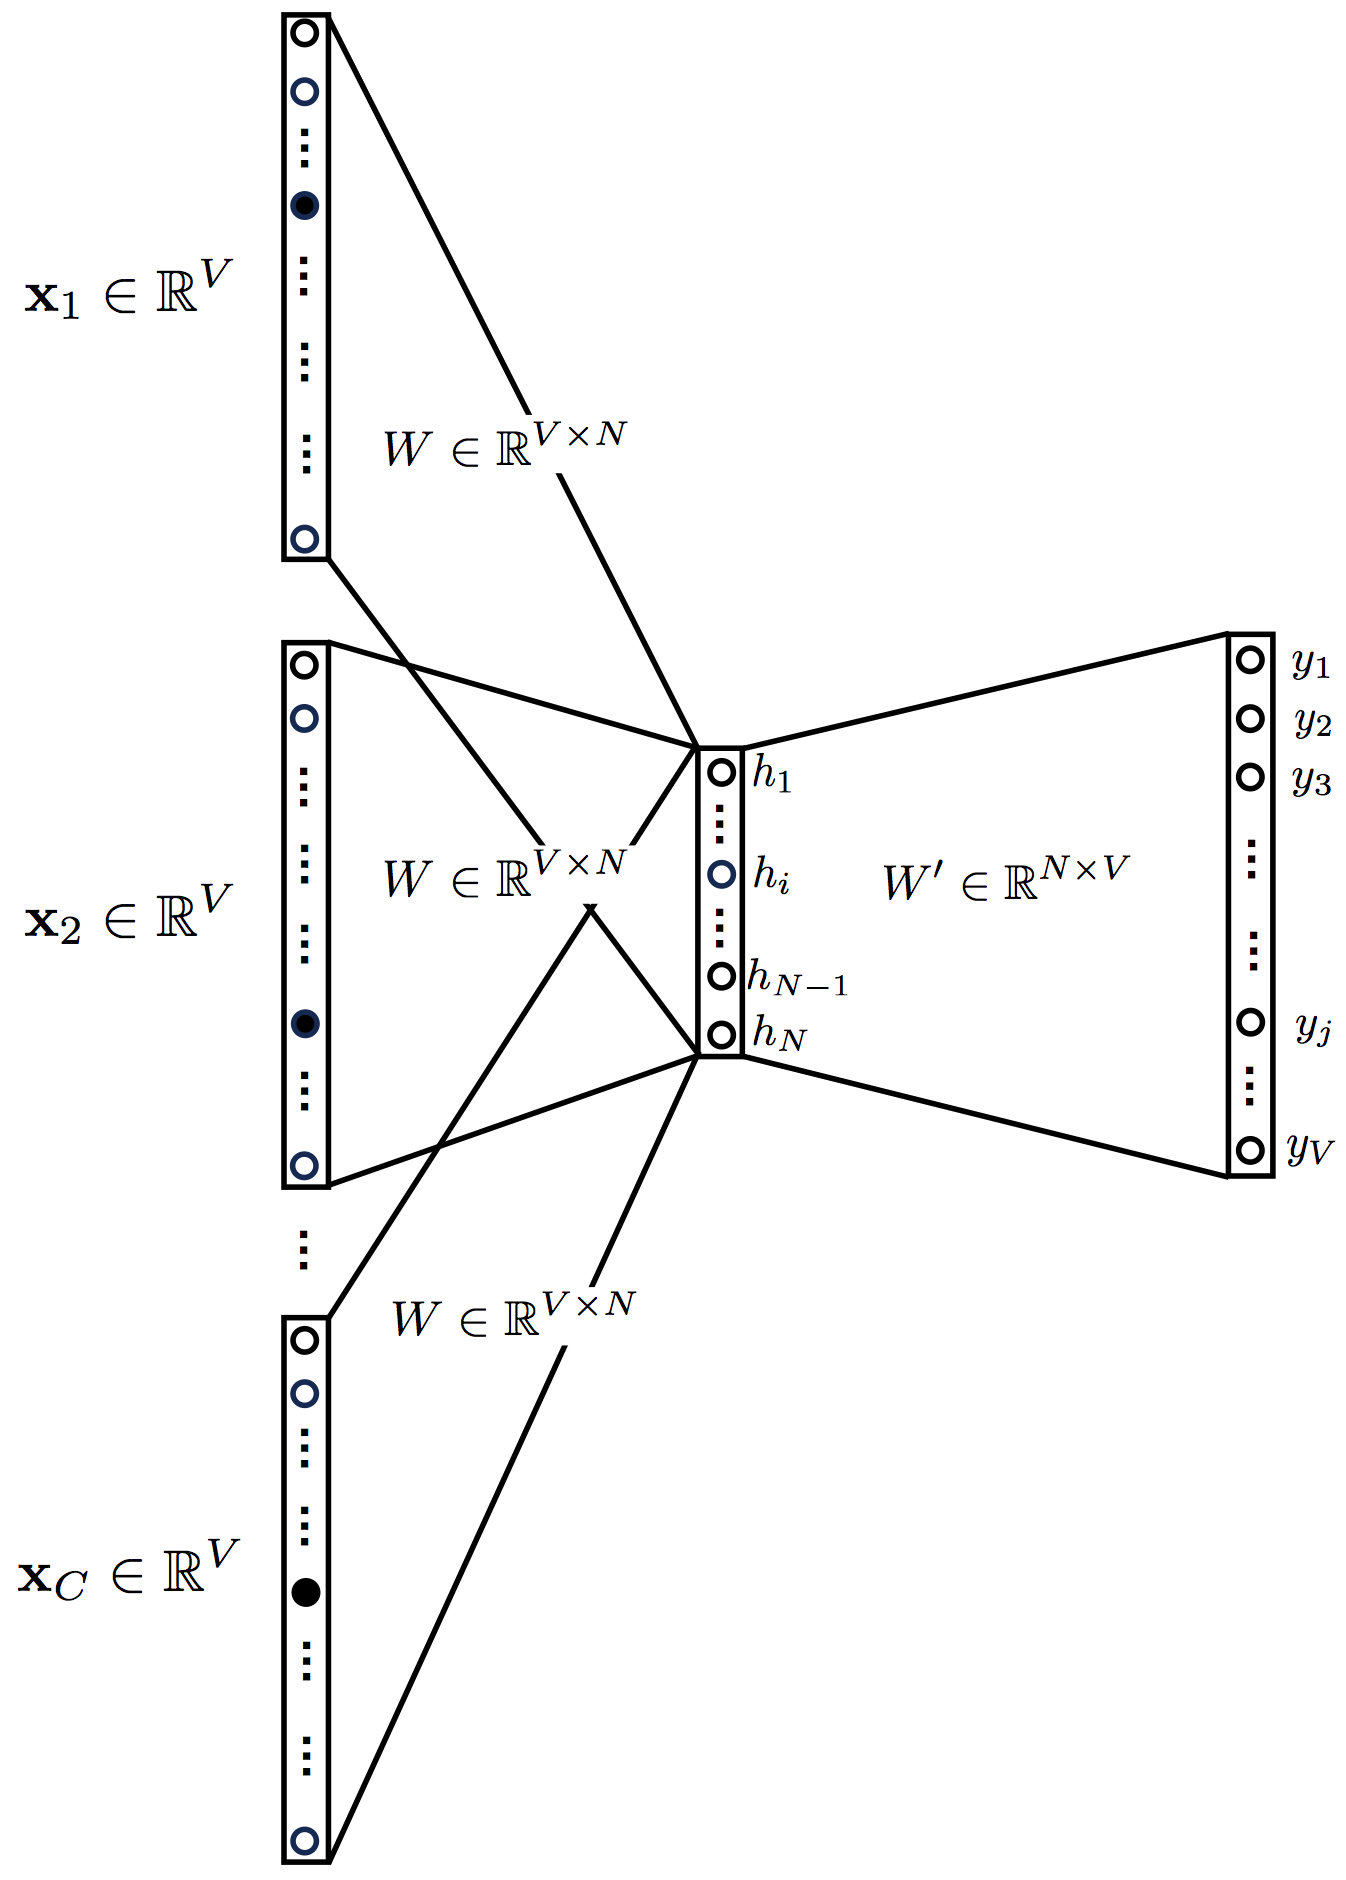
\includegraphics[width=0.85\linewidth]{image/Cbow} \\ а)}
	\end{minipage}
	\hfill
	\begin{minipage}[h]{0.49\linewidth}
		\center{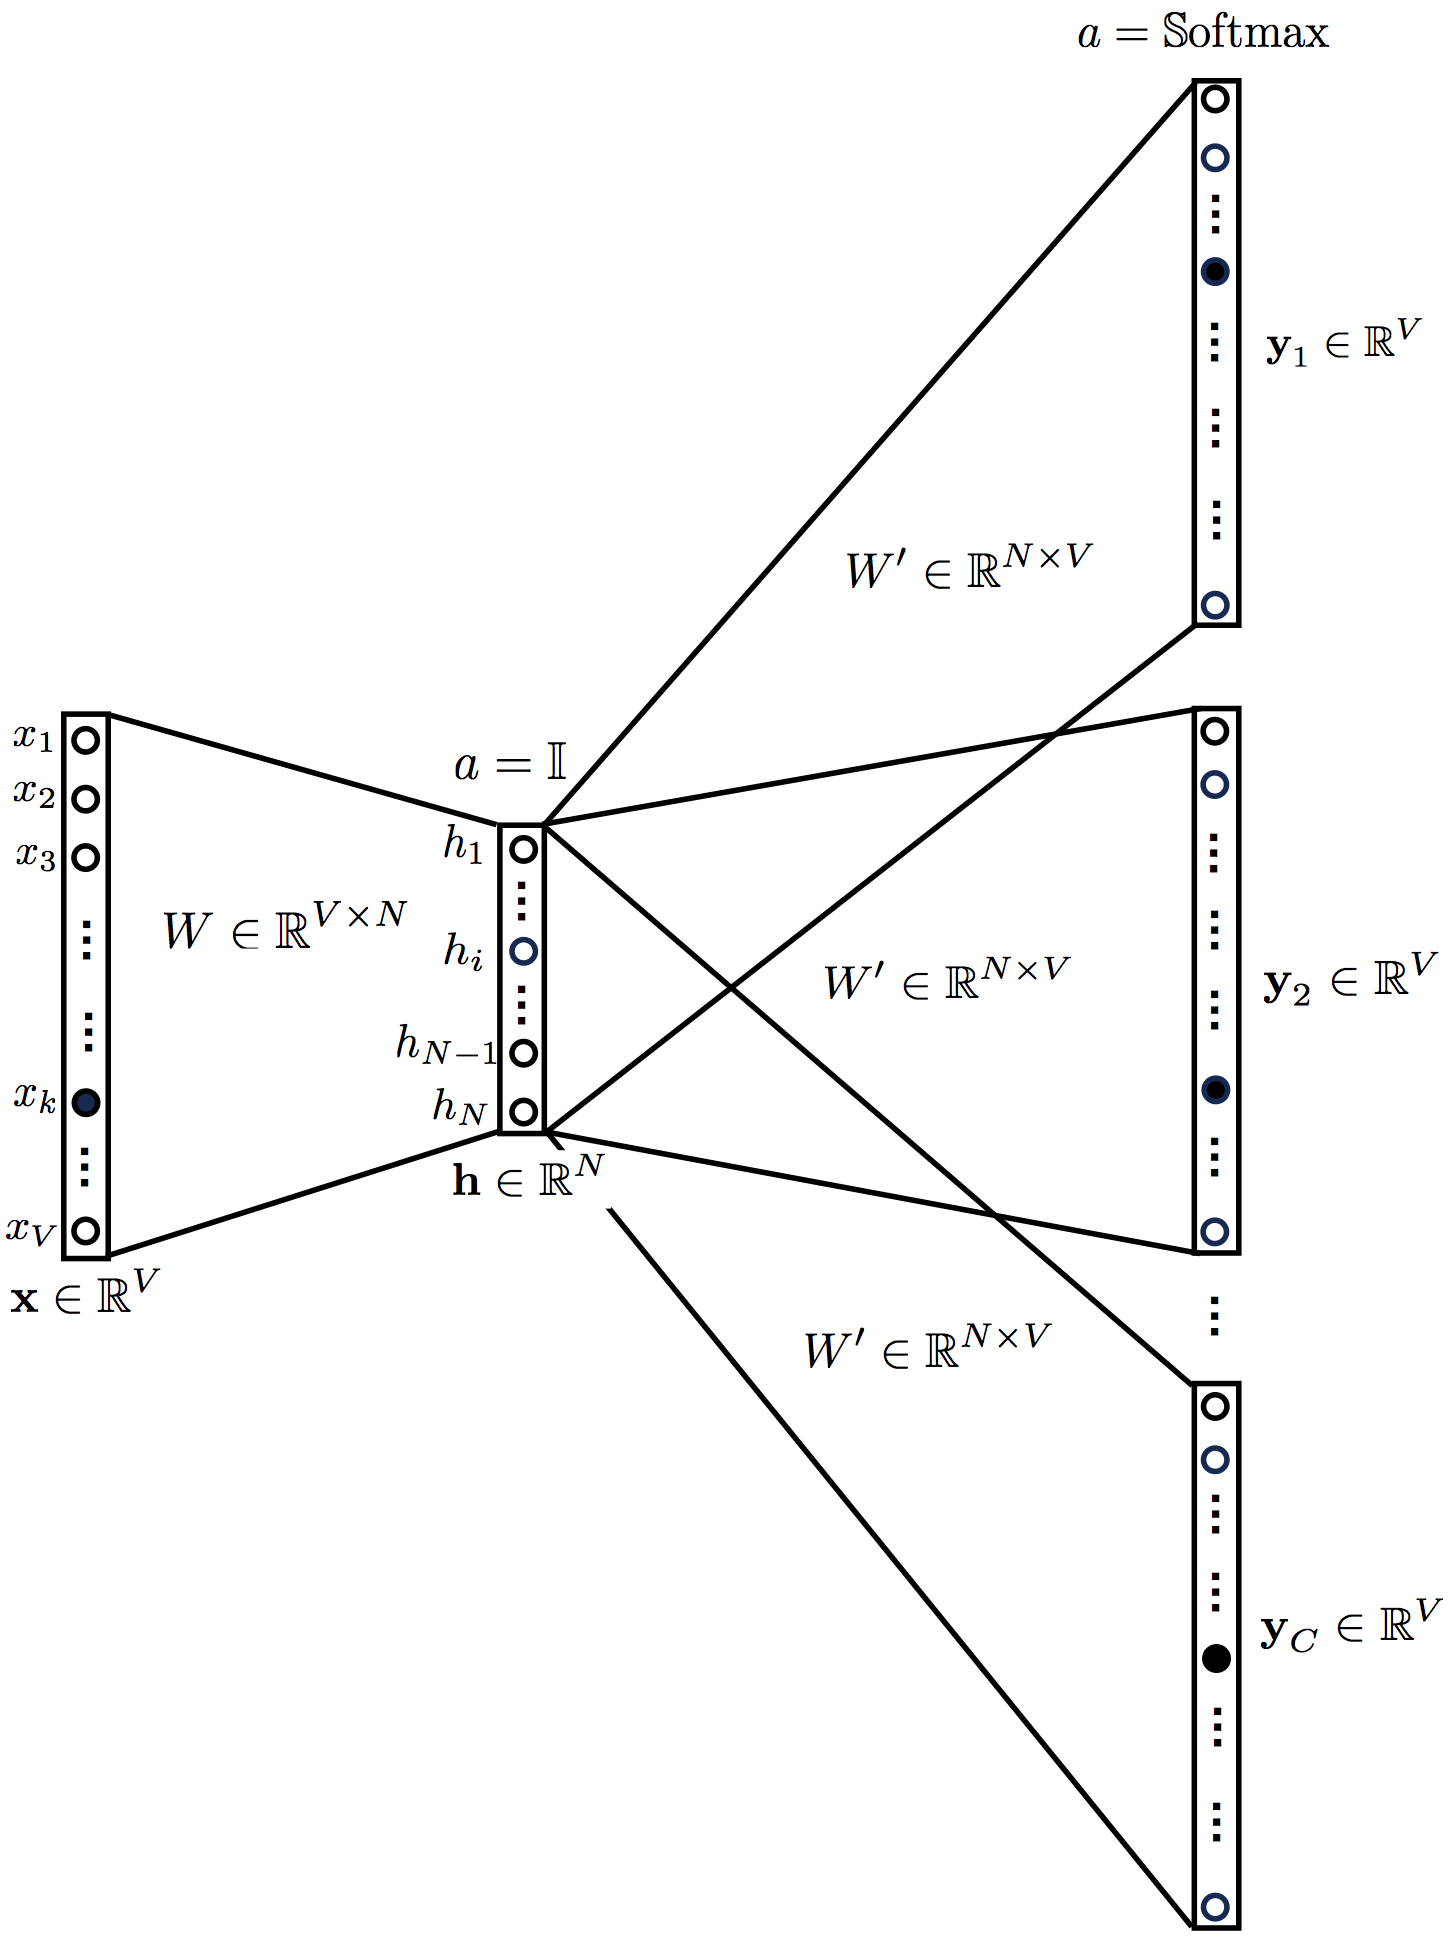
\includegraphics[width=0.85\linewidth]{image/Skip-gram} \\ б)}
	\end{minipage}
	\caption{Схемы архитектур CBOW (a), Skip-gram (б)}
	\label{fig:word2vec}
\end{figure}

Архитектуры представляют из себя полносвязные нейронные сети с обратным распространением ошибки.
Для больших словарей метод активации softmax накладывает серьезные вычислительные нагрузки.
При работе softmax каждое слово  представляет из себя отдельный класс, авторы word2vec предложили использовать бинарную классификацию вместо многоклассовой.
Предлагается научить модель отличать пары слов, которые встречаются в одном контексте, от тех, которые никогда не стоят в одном контексте.

Появление модели word2vec послужило мощным толчком для развития моделей обработки естественного языка.

%Continuous Bag-of-Words дословно переводится как <<непрерывный мешок слов>>.
%Работает архитектура похожим образом, предсказывается вероятность появления слова по его контексту в виде окна фиксированного размера.
%Архитектура Skip-gram наоборот предсказывает вероятность появления контекста у заданного слова.
%Порядок слов в контексте не влияет на результат ни в одном из этих алгоритмов.
%В процессе обучения модель корректирует веса между входным и скрытым слоем, которые в дальнейшем станут эмбеддингами слов.

\subsection{FastText}

FastText \cite{ft} является продолжением развития модели word2vec.
FastText имеет архитектуру Skip-gram.
При этом в fastText отличается от word2vec тем, что у новой модели используются N-граммы символов.
Например, для слова молоко 3-граммами являются <мо, мол, оло, лок, око, ко>, где символы << < >> и << > >> кодируют начало и конец слова соответственно.
Векторные представления строятся именно для N-грамм, векторные представления слов - это сумма векторных представлений всех его N-грамм.
При этом решается проблема того, что словарь модели word2vec был ограничен и не все формы слов вошли в словарь.
Также, использование N-грамм позволяет получать векторные представления для редких слов.

В русском языке существуют слова омонимы и омографы, слова, которые совпадают в написании, но имеют разный смысл.
Предыдущие методы обработки естественного языка никак не решали эту проблему.
Одной из первых эту проблему постаралась решить модель ELMo.

\subsection{ELMo}

ELMo (Embeddings from Language Models) -- модель обработки естественного языка, которая представляет собой двунаправленную рекуррентную нейронную сеть с LSTM.
Модель была предложена в работах \cite{elmo1,elmo2,elmo3}.
Модель учитывает семантическую неоднозначность слов в предложениях, и эмбеддинги, присваиваемые словам, зависят не только от самого слова, но и от контекста.
Основная идея получения эмбеддингов -- использование скрытых состояний LSTM.
Разберемся по подробнее с LSTM блоками.

\subsubsection{LSTM}

LSTM или Long short-term memory были предложены в статье \cite{lstm}.
Название блоков дословно переводится, как долгая краткосрочная память.
Данные блоки являются разновидностью архитектуры рекуррентных нейронных сетях и предназначены для того, чтобы хранить информацию на длинные и короткие промежутки времени.

Данные блоки имеют одну особенность, в них нет функции активации.
За счет этого хранимая информация не размывается по времени и во время обучения при использовании метода обратного распространения ошибки вычисляемый градиент не исчезает.

В LSTM модуле есть 2 основных компонента: состояние ячейки и различные фильтры.
Состояние ячейки -- это память сети, которая передается по всей цепочке.

Во время обучения состояние ячейки постоянно меняется. Происходит добавление и удаление информации.
Все это контролируют фильтры.
Фильтры состоят из сигмоидальной нейронной сети и операции поточечного умножения.
Сигмоидальный модуль возвращает числа в диапазоне [0;1], которые обозначают долю блока информации, которую следует пропустить дальше по сети.
Фильтры бывают трех типов:
\begin{enumerate}
	\itemsep0em 
	\item Забывания;
	\itemsep0em 
	\item Входные;
	\itemsep0em 
	\item Выходные.
\end{enumerate}

На рисунке \ref{fig:LSTM_layers}.а изображен фильтр забывания.
На данном этапе решается какую информацию можно забыть или оставить.
$h_{t-1}$ -- значения выхода из предыдущего блока, $x_t$ -- вход данного блока.
Данные значения проходят обработку в сигмоидальном блоке.
Результаты находятся в диапазоне [0;1].
То, что ближе к 0 будет забыто, что ближе к 1 оставлено (\ref{fraq:forget}).


\begin{equation}
	f_t = \sigma(W_f\cdot[h_{t-1},x_t] + b_f)
	\label{fraq:forget}
\end{equation}

На рисунке \ref{fig:LSTM_layers}.б решается какая информация будет храниться в состоянии ячейки.
Сигмоидальный блок решает какую информацию необходимо обновить (\ref{fraq:enter_sigma_i}), tanh-слой строит вектор со значениями, которые могут быть добавлены в состояние ячейки (\ref{fraq:enter_sigma}). 

\begin{equation}
	i_t = \sigma(W_i\cdot[h_{t-1},x_t] + b_i) 
	\label{fraq:enter_sigma_i}
\end{equation}
\begin{equation}
	\tilde C_t = \tanh(W_C\cdot[h_{t-1},x_t] + b_C)
	\label{fraq:enter_sigma}
\end{equation}

На рисунке \ref{fig:LSTM_layers}.в проиллюстрирован процесс изменения состояния ячейки.
Ненужная информация в $C_{t-1}$ забывается после умножения на $f_t$.
Затем к состоянию ячейки добавляются текущие изменения $i_t * \tilde C_t$.
Все вместе можно записать формулой (\ref{fraq:changes_sigma}).

\begin{equation}
	\tilde C_t = f-t * C_{t-1} + i_t * \tilde C_t
	\label{fraq:changes_sigma}
\end{equation}



\begin{figure}[H]
	\begin{minipage}[h]{0.4\linewidth}
		\center{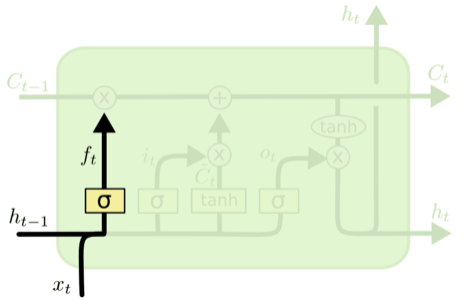
\includegraphics[width=1\linewidth]{image/LSTM_1}} а) \\
	\end{minipage}
	\hfill
	\begin{minipage}[h]{0.4\linewidth}
		\center{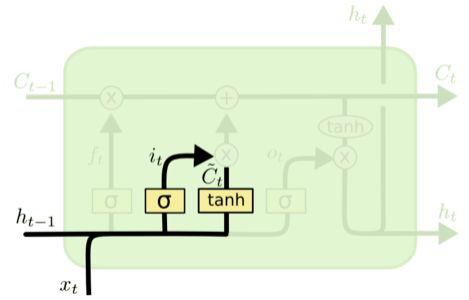
\includegraphics[width=1\linewidth]{image/LSTM_2}} \\б)
	\end{minipage}
	\vfill
	\begin{minipage}[h]{0.4\linewidth}
		\center{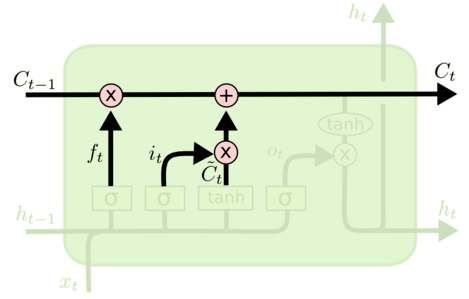
\includegraphics[width=1\linewidth]{image/LSTM_3}} в) \\
	\end{minipage}
	\hfill
	\begin{minipage}[h]{0.4\linewidth}
		\center{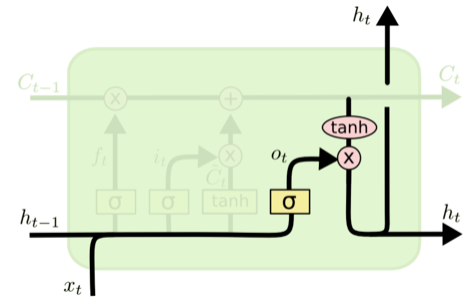
\includegraphics[width=1\linewidth]{image/LSTM_4}} г) \\
	\end{minipage}
	\caption{Виды фильтров: 
		 a) слой фильтра забывания,
		 b) слой входного фильтра,
		 c) применение текущих изменений,
		 d) слой выходного фильтра.}
	\label{fig:LSTM_layers}
\end{figure}

На рисунке \ref{fig:LSTM_layers}.г изображено формирование выходов.
Сначала в сигмоидальном слое поступает информация предыдущего выхода $h_{t−1}$ и текущего входа $x_t$, где определятся какая информация из состояния ячейки будет отправлена на выход (\ref{fraq:out_sigma_o}).
Далее значения из состояния ячейки обрабатываются tanh-слоем и перемножаются со значениями с сигмоидального слоя (\ref*{fraq:out_sigma}).

\begin{equation}
	o_t = \sigma(W_o\cdot[h_{t-1},x_t]) 
	\label{fraq:out_sigma_o}
\end{equation}
\begin{equation}
	\tilde h_t = o_t * \tanh(C_t)
	\label{fraq:out_sigma}
\end{equation}

После преобразований $h_t$ и $C_t$ передаются на следующий блок по цепочке.	

\subsubsection{Структура ELMo}

Архитектура ELMo представлена на рисунке \ref{fig:elmostructure}.а.
ELMo состит из двух двухслойных разнонаправленных рекуррентных LSTM сетей.
Было замечено, что верхние слои LSTM сети отвечают за семантический смысл слова, а нижние -- за синтаксис и грамматику.

\begin{figure}[H]
	\begin{minipage}[h]{0.499\linewidth}
		\center{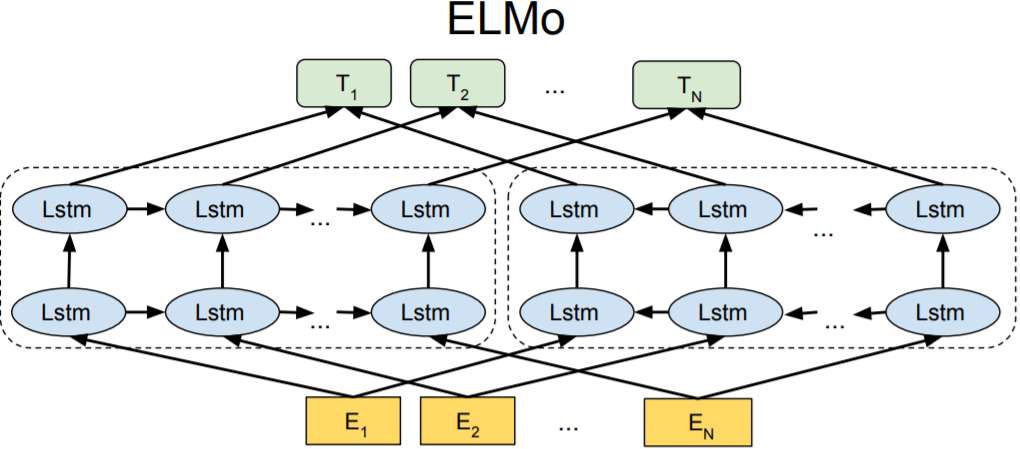
\includegraphics[width=1\linewidth]{image/elmo_structure} \\ а)}
	\end{minipage}
	\hfill
	\begin{minipage}[h]{0.499\linewidth}
		\center{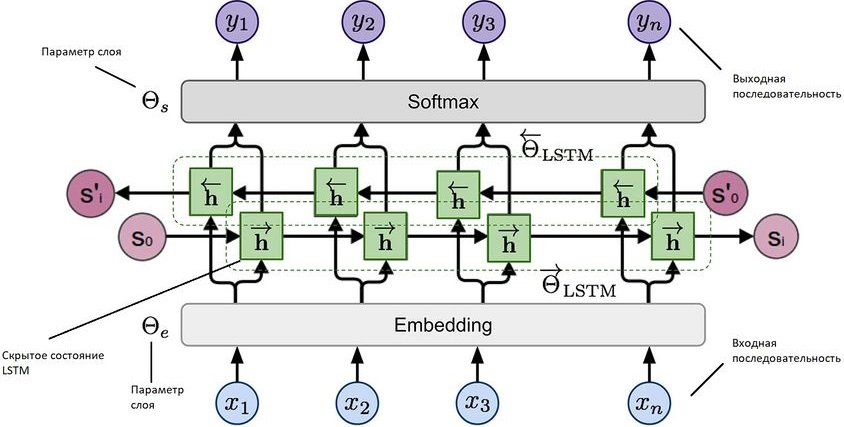
\includegraphics[width=1\linewidth]{image/900px-ElmoExplain} \\ б)}
	\end{minipage}
	\caption{Архитектура модели ELMo (а), принцип работы модели ELMo (б)}
	\label{fig:elmostructure}
\end{figure}

На рисунке \ref{fig:elmostructure}.б схематично изображен принцип работы модели ELMo.
Пусть на вход подаются токены $t_1, ...., t_N$, на которые разделено предложение.
Будем считать логарифм правдоподобия метки слова в обоих направлениях, учитывая контекст справа и слева от слова.
Так модель предсказывает вероятность следующего токена с учетом истории.

Пусть есть $L$ слоев сети, входные и выходные данные представляются в виде векторных представлений слов.
Каждый результирующий вектор будет считаться на основании множества (\ref{fraq:array_elmo}).

\begin{equation}
	\left\{ x_k^{LM}, \overrightarrow{h_{k,j}^{LM}}, \overleftarrow{h_{k,j}^{LM}}  |j = 1, ...,L\right\} = 
	\left\{h_{k,j}^{LM}|j = 1, ...,L
	\right\}
	\label{fraq:array_elmo}
\end{equation}

где $x_k^{LM}$ -- входящий токен, $\overrightarrow{h_{k,j}^{LM}}, \overleftarrow{h_{k,j}^{LM}}$ -- скрытые слои в обоих направлениях.

Результатом работы ELMo будет выражение (\ref{fraq:elmo_result}).

\begin{equation}
	ELMO_k^{task} = \gamma^{task}\sum_{j=0}^{L} s_{i}^{task}h_{k,j}^{LM}
	\label{fraq:elmo_result}
\end{equation}

где $\gamma^{task}$ -- масштабирующий коэффициент, который регулирует то, как могут отличаться по норме ембеддинги слов, $s_{i}^{task}$ -- обучаемые параметры, нормализованные функцией softmax.

Векторным представлением слова будет яаляться взвешенная сумма значений на всех скрытых слоях ELMo.

Вскоре после выхода ELMo появилась еще одна мощная контекстуализированная модель, называется она BERT.

\subsection{BERT}

BERT \cite{bert1} или Bidirectional Encoder Representations from Transformers -- модель обработки естественного языка выпущенная в 2018 году командой Google AI.
В основе работы модели лежит ряд недавних разработок в сфере обработки естественного языка.
Можно выделить разработки Semi-supervised Sequence learning \cite{semi}, уже упомянутый ELMo \cite{elmo1,elmo2,elmo3}, ULMFiT \cite{ulmfit}, OpenAI Transformer \cite{transformers} и Transformer \cite{attention}.

Принцип работы модели BERT основан на применении кодировщиков (encoders) из Transformer.
Рассмотрим подробнее принцип работы кодировщиков.

\subsubsection{Encoder from Transformer}

Кодировщик -- это составная часть модели трансформера, подробно он опсисан в статье \cite{attention}.
%Для того, чтобы разобраться с кодировщиком 
Принцип работы модели трансфомера основан на механизме внутреннего внимания.
Работа модели состоит в том, что модель принимает на вход предложение на одном языке и выводит на другом.
Другими словами, осуществляется перевод предложения с одного языка на другой.

Важным преимуществом модели трансформера является то, что все вычисления могут выполняться параллельно, в том числи и при использовании TPU.

Модель состоит из двух компонентов: кодирующего и декодирующего.
Предложение сначала попадает в кодирующий компонент, далее передается в декодирующий компонент, на выходе из декодирующего компонента получается переведенное предложение.

Каждый компонент состоит из более мелких модулей (рисунок \ref{fig:bertgroups}).
Кодирующий компонент состоит из кодировщиков (encoders), декодирующий -- из декодировщиков (decoders).
По структуре все модули в каждом компоненте идентичны, разницу составляют только веса, получаемые при обучении модели.
Количество модулей в каждом компоненте одинаковое.

\begin{figure}[H]
	\centering
	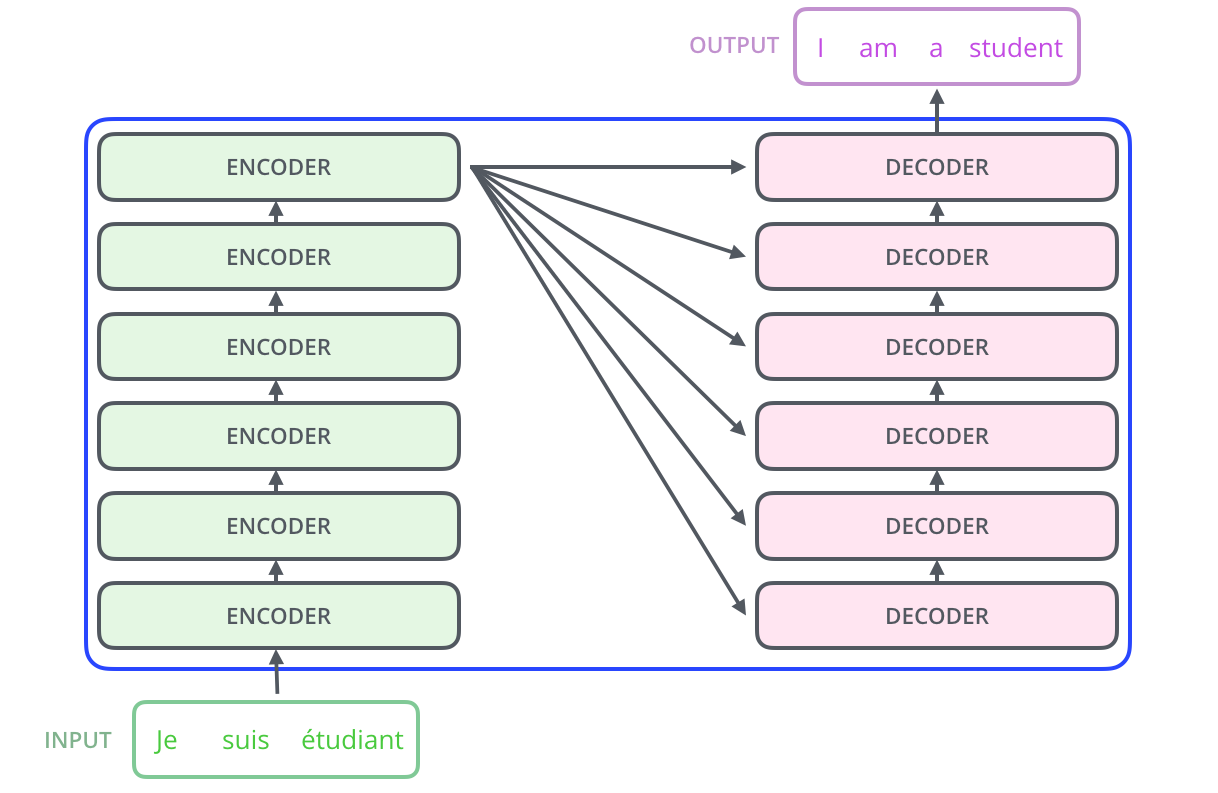
\includegraphics[width=0.6\linewidth]{image/bert_groups}
	\caption{Структура модели Transformer}
	\label{fig:bertgroups}
\end{figure}


Кодировщик состоит из двух подслоев (рисунок \ref{fig:bertencdec}).
Первый слой -- слой внутреннего внимания (self-attention), данный блок помогает модели работать с контекстом во время кодирования слова, подробнее механизм работы разберем позже.
Второй слой -- нейронная сеть прямого распределения (feed-forward neural network).
По сути, второй слой представляет из себя полносвязную нейронную сеть, применяемую к каждому слову в отдельности.

Декодировщик состоит из тех же слоев (рисунок \ref{fig:bertencdec}), но с одним исключением.
Между слоем внутреннего внимания и слоем прямого распределения стоит слой внимания (Encoder-Decoder Attention), который помогает декодеру 	сосредотачиваться на более значимых частях предложения.

\begin{figure}[H]
	\centering
	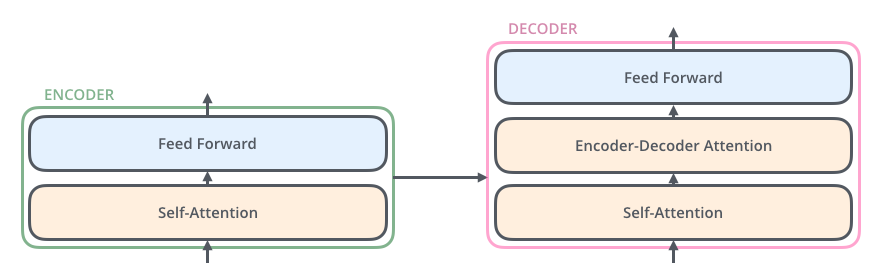
\includegraphics[width=0.8\linewidth]{image/bert_enc_dec}
	\caption{Структура кодировщика и декодировщика}
	\label{fig:bertencdec}
\end{figure}

Рассмотрим алгоритм работы блока кодировщика.
На вход блоку подается информация с выхода предыдущего блока, в случае первого блока, на вход подаются неконтекстуализированные эмбеддинги слов.
Эмбеддинги слов попадают в слой внутреннего внимания.

%Разберем принцип работы слоя внутреннего внимания.
Векторные представления слов подаются в виде матрицы $X$ размером $L*N$, где $L$ -- длина векторного представления, $N$ - количество слов в предложении.

Первый этап -- это создание трех матриц, матриц запроса (\ref{fraq:elmo_self_Q}), ключа (\ref{fraq:elmo_self_K}) и значения (\ref{fraq:elmo_self_V}).

\begin{equation}
	Q = X * W_Q
	\label{fraq:elmo_self_Q}
\end{equation}
\begin{equation}
	K = X * W_K
	\label{fraq:elmo_self_K}
\end{equation}
\begin{equation}
	V = X * W_V
	\label{fraq:elmo_self_V}
\end{equation}

где $X$ -- матрица эмбеддингов слов,
$Q, K, V$ -- матрицы запроса ключа и значения соответственно,
$W_Q, W_K, W_V$ -- матрицы весов, получаемые в процессе обучения моделей.

Следующим шагом необходимо получить для каждого слова в предложении коэффициент схожести $S$ со всеми словами в этом же предложении (\ref{fraq:elmo_self_score}).
Далее полученные коэффициенты делятся на корень из размерности векторного представления $\sqrt{L}$ для получения более стабильного градиента.
После этого полученные значения пропускают через функцию softmax для нормирования весов (\ref{fraq:elmo_self_softmax}).
Наибольшие коэффициенты будут у слов самим с собой, это нормально.
На данном этапе необходимо определить какие из слов в предложении несут похожую смысловую нагрузку.
Чем больше значение коэффициента, тем больше слова похожи друг на друга.
Влияние нерелевантных слов необходимо свести к минимуму, подобрав им минимальные веса.
Далее полученные веса $M$ умножаются на матрицу значений $V$ (\ref{fraq:elmo_self_Z}) и складываются.
Полученная взвешенная сумма $Z$ для каждого слова будет результатом работы слоя внутреннего внимания.

\begin{equation}
	S = Q * K^T
	\label{fraq:elmo_self_score}
\end{equation}

\begin{equation}
	M = softmax(\dfrac{S}{\sqrt{L}})
	\label{fraq:elmo_self_softmax}
\end{equation}

\begin{equation}
	Z =  M * V
	\label{fraq:elmo_self_Z}
\end{equation}

Если объединить все выражения (\ref{fraq:elmo_self_score}) -- (\ref{fraq:elmo_self_Z}), то получится следующее (\ref{fraq:elmo_self_all}).

\begin{equation}
	Z =  softmax(\dfrac{Q * K^T}{\sqrt{L}}) * V
	\label{fraq:elmo_self_all}
\end{equation}

Данный метод внутреннего внимания совершенствуется добавлением механизма под названием: множественное внимание (multi-head attention).
Этот прием позволяет улучшить производительность внутреннего слоя за счет повышения способности модели фокусироваться на разных позициях.
При этом создается несколько подпространств со своими случайно сгенерированными матрицами запроса, ключа и значения.
В модели трансформера используется 8 подпространств.

Результатом работы этих 8 подпространств внутреннего внимания будут 8 матриц весов $Z$.
Для того, чтобы не увеличивать размерность данных предлагается конкатенировать все матрицы $Z$ и умножить их на еще одну матрицу весов $W_O$.

Важная часть обработки естественного языка -- обработка порядка слов во входящем предложении.
В модели трансформер эта проблема решается путем добавления вектора позиционного кодирования.
Эти вектора имеют определенный шаблон и добавляются к каждому входящему эмбеддингу.
Позиционное кодирование позволяет определить позицию каждого слова или расстояние между словами в предложении.
Идея метода в том, что добавление векторов к эмбеддингам создает осмысленное расстояние между векторными представлениями в процессе проецирования в $Q/K/V$ векторы и скалярного произведения при вычислении внимания.

В приложении А представлена визуализация одного из методов позиционного кодирования.
Каждая строка -- это один вектор, первому слову соответствует первая строка, второму -- вторая и так далее.
По центру есть разрыв, значения слева и справа сгенерированы разными функциями, слева используется функция с синусом, справа с косинусом.

Декодеры работают по-похожему принципу с небольшими изменениями.
В слое внутреннего внимания скрываются все эмбедднги, следующие за целевым векторным представлением.
Упомянутый ранее промежуточный слой внимания Encoder-Decoder attention, помимо взвешенных сумм со слоя внутреннего внимания, принимает на вход матрицы ключей и значений ($K,V$) с выхода последнего кодировщика.

Во время обучения данные проходят по всему маршруту и результат сравнивается с эталонным.
Все матрицы весов изначально задаются случайными значениям и подбираются методом обратного распространения ошибки.

\subsubsection{Структура BERT}

В модели BERT для векторного представления слов используются только кодировщики.
Структура модели представлена на рисунке \ref{fig:bertstructure}.
Модель состоит из 12 кодировщиков.

\begin{figure}[H]
	\centering
	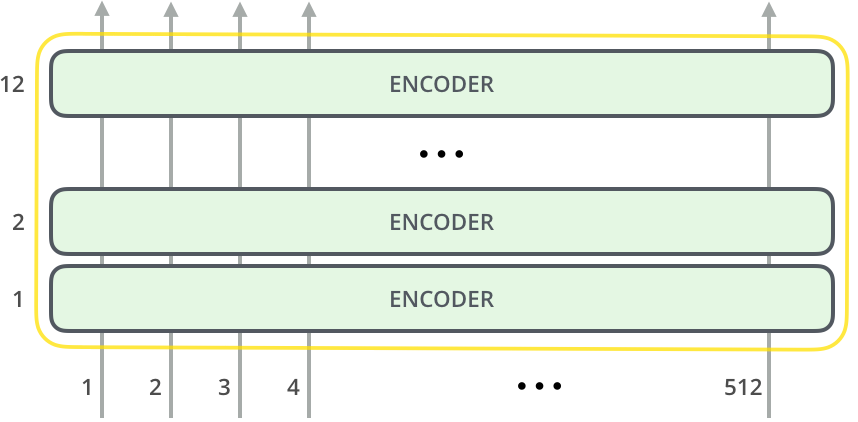
\includegraphics[width=0.5\linewidth]{image/bert_structure}
	\caption{Структура модели BERT}
	\label{fig:bertstructure}
\end{figure}

В процессе работы модель BERT принимает на вход по аналогии с трансформером набор слов, при этом в начало текста помещается специальный токен \textit{[CLS]}, в конец каждого предложения помещается токен \textit{[SEP]} для разграничения предложений.

При этом выход модели существенно отличается от трансформера.
Трансформер выдает готовое переведенное предложение.
BERT имеет на выходе только эмбеддинги слов, которые в последствии можно использовать в различный моделях машинного обучения, например, для задачи классификации текстов.

Модель BERT обучена для решения двух задач.
Первая задача состоит в том, чтобы предсказывать пропущенные слова в предложении.
Модель обучалась на текстах, в которых было скрыто 15\% слов.
Вторая задача заключается в том, чтобы определить насколько одно предложение является логичным продолжением второго.

Важным преимуществом модели BERT стало то, что при обучении не требуется размеченный датасет.
Модель способна сама подготовить себе данные для обучения.
Это позволило разработчикам обучить модель на больших объемах данных.

\subsection{Исследование методов оценки аффинных преобразований}

В основе большинства методов оценки аффинных преобразований лежит описанное в формуле (\ref{eq:cos_sim}) косинусное сходство.
Для удобства применяется также косинусное расстояние (\ref{eq:cos_dist}).

\begin{equation}
	similarity(A,B) = cos(A,B) = cos(\theta) = \dfrac{A\cdot B}{\|A\| \|B\|}
	\label{eq:cos_sim}
\end{equation}

\begin{equation}
	distance(A,B) = 1 - similarity(A,B)
	\label{eq:cos_dist}
\end{equation}

Аффинные преобразования над векторными представлениями слов предполагают задачу пропорциональной аналогии.
Задача пропорциональной аналогии заключается в том, чтобы установить для группы пар слов определенную логическую связь в парах.
Рассмотрим группу пар слов $(a: a^*), (b: b^*)$. 
Известно, что слова в первой группе относятся друг к другу также, как и слова во второй группе.
Представить это можно следующим образом (\ref{eq:preobr}).

\begin{equation}
	(a: a^*) :: (b: b^*)
	\label{eq:preobr}
\end{equation}

Если в парах действует одна и та же связь, то можно выразить одно из слов через 3 других слова (\ref{eq:yravn}).

\begin{equation}
	y = v_b - v_a + v_{a^*}
	\label{eq:yravn}
\end{equation}

где 
$y$ - искомый вектор,
$v_x$ - эмбеддинг для слова $x$.

Но вектору $y$ может не соответствовать ни одного слова, поэтому в качестве ответа берется ближайшее слово к $y$.
Для корректно работающей модели ответ совпадет с $b^*$.
Результат можно выразить формулой (\ref{eq:3cosadd}).

\begin{equation}
	y^* = \underset{v \notin \{v_b, v_a, v_{a^*}\}}{argmax} \; cos(v, v_b - v_a + v_{a^*})
	\label{eq:3cosadd}
\end{equation}


%Возникает необходимость оценить в качество решения задачи пропорциональной аналогии.
Интуитивно понятным способом оценить качество будет сопоставить все пары слов друг с другом, посчитать одно из слов по формуле (\ref{eq:3cosadd}) \cite{21} и найти среднее значение косинусной близости после трансформаций.
Данный способ получил название \textbf{3CosAdd}.

Существует пердположение, что \ref{eq:3CosMul} эквивалентно (\ref{eq:3cosadd}). Этот метод получил название \textbf{3CosMul} \cite{21}.

\begin{equation}
	y^* = \underset{v \notin \{v_b, v_a, v_{a^*}\}}{argmax} \; cos(v, v_{a^*}) - cos(v, v_a) + cos(v, v_b)
	\label{eq:3CosMul}
\end{equation}

Если в группе у пар одна и та же связь, то можно посчитать среднюю разницу между векторами в парах и задача аналогии будет решаться через посчитанную разницу.
Эта идея предлагается в метрике	\textbf{3CosAvg} (\ref{eq:3CosAvg}) \cite{28}.

\begin{equation}
	y^* = \underset{v \notin \{v_b, v_a, v_{a^*}\}}{argmax} \; cos(v,v_b + \dfrac{\sum_{i=1}^{n}v_{a_i^*}}{n} - \dfrac{\sum_{i=1}^{n}v_{a_i}}{n})
	\label{eq:3CosAvg}
\end{equation}

Существуют и другие методы оценки аффинных преобразований.
Метод \textbf{Only-b} \cite{27} основан на предположении, что вектора $v_b$ и $v_{b^*}$ находятся максимально близко друг к другу (\ref{eq:Only-b}).

\begin{equation}
	y^* = \underset{v \notin \{v_b, v_a, v_{a^*}\}}{argmax} \; cos(v, v_b)
	\label{eq:Only-b}
\end{equation}

В методе \textbf{Ignore-a} \cite{27} предполагается, что результат ближе всего к сумме векторов $v_b$ и $v_{a^*}$ (\ref{eq:Ignore-a}).

\begin{equation}
	y^* = \underset{v \notin \{v_b, v_a, v_{a^*}\}}{argmax} \; cos(v, v_b + v_{a^*})
	\label{eq:Ignore-a}
\end{equation}

В методе \textbf{Add-opposite} \cite{27} результатом является вектор, ближайший к выражению $-(v_{a^*} - v_a) + v_b$ (\ref{eq:Add-opposite}).

\begin{equation}
	y^* = \underset{v \notin \{v_b, v_a, v_{a^*}\}}{argmax} \; cos(v, -(v_{a^*} - v_a) + v_b)
	\label{eq:Add-opposite}
\end{equation}

Метод \textbf{MULTIPLY} \cite{27} имеет следующий вид (\ref{eq:MULTIPLY}).

\begin{equation}
	y^* = \underset{v \notin \{v_b, v_a, v_{a^*}\}}{argmax} \; \dfrac{cos(v, v_{a^*}) \; cos(v, v_b)}{cos(v, v_a)}
	\label{eq:MULTIPLY}
\end{equation}


\newpage

\section{Теоретическая часть}

\subsection{Постановка задачи}

Необходимо исследовать возможность и оценить качество аффинных преобразований при решении задачи пропорциональной аналогии в семантическом пространстве контекстуализированной модели векторного представления слов.

Пусть имеется множество слов $W$ мощностью $L$. Каждому слову $w \in W$ соответствует множество векторных представлений $V_w = \{v_{1w}, v_{2w}, ..., v_{nw}\}| V_w \subset V$, где $v_{iw}$ -- векторное представление слова $w$ в $i$-ом контексте, $V$ множество всех векторных представлений слов.
При этом существует функция $\eta$, которая преобразует множество эмбеддингов слова в векторное представление $v_w' = \eta(V_w) | v_w' \in V'$.

Выделим пары слов $(w_{11},w_{12}), (w_{21},w_{22}), ..., (w_{k1},w_{k2})$ из множества слов $W$, где $w_{ij}$ -- $j$-ое слово в паре под номером $i$.
Все пары подобраны таким образом, что в них действует одно и то же семантическое отношение $R:w_{i1} \rightarrow w_{i2}$.
Это означает, что можно можно составить пропорциональные аналогии слов: $(w_{i1}, w_{i2})::(w_{j1}, w_{j2}), i \neq j$.
Каждой паре слов можно сопоставить пары векторов $(v_{11}',v_{12}'), (v_{21}',v_{22}'), ..., (v_{k1}',v_{k2}')$, где $v_{ij}'$ -- $j$-ый вектор в паре под номером $i$. .
В итоге получаются следующие выражения:

\begin{align*}
&w \in W, |W| = L\\
&V_w = \{v_{1w}, v_{2w}, ..., v_{nw}\}| V_w \subset V\\
&v'_w = \eta(V_w)\\
&v'_w \in V', |V'| = L\\
&f : W \rightarrow V'\\
&P = \{(w_{i1}, w_{i2})|w_{i1}, w_{i2} \in W, i=\overline{1,k}\}\\
&R:w_{i1} \rightarrow w_{i2}\\
&V_P' = \{(v'_{i1}, v'_{i2})|v'_{i1}, v'_{i2} \in V', i=\overline{1,k}\}\\
&g = P \rightarrow V_P'
\end{align*}

Аффинное преобразование -- это отображение пространства в себя, при котором параллельные прямые переходят в параллельные прямые, пересекающиеся -- в пересекающиеся, скрещивающиеся -- в скрещивающиеся.

Математически аффинное преобразование $\phi : \mathbb{R}^n \rightarrow \mathbb{R}^n$ выглядит выглядит как в выражении (\ref{fraq:aff_matr}).

\begin{equation}
	\phi(x) = M \cdot x + v
	\label{fraq:aff_matr}
\end{equation}

где $M$ -- обратимая матрица, $v \in \mathbb{R}^n$.

Аффинные преобразования бывают разных видов: движения, растяжения и подобия.
Задача пропорциональной аналогии относится к движению, типу аффинного преобразования, при котором сохраняются расстояния между любыми двумя точками.
Математическая запись пропорциональной аналогии выглядит следующим образом:

$$\phi(x) =  x + v$$

Сформированная пара векторов $(v_{i1}', v_{i2}'), i = \overline{1,k}$ является парой радиус-векторами для точек $A_{i1}, A_{i2}$.
Необходимо установить существование аффинного преобразования, при котором все точки $A_{i1}$ будут соответствовать точкам $A_{i2}$.

$$v_{i2}' = v_{i1}' + d$$

Это означает, что расстояние между любыми двумя точками $A_{i1}, A_{j1}, i \neq j$ будет точно таким же, как и между любыми двумя точками $A_{i2}, A_{j2}, i \neq j$.
Но вероятность того, что при параллельном переносе попадется точка, для которой существует радиус вектор $v_r' \in V'$, крайне мала.

Однако есть решение, можно взять вектор максимально близкий к искомому, то есть для вектора $v_r'' \notin V'$ сопоставить вектор  $v_r' \in V'$:

$$v_{i2}'' = v_{i1}' + d$$

С ограничением:

$$v_{i2}' = \underset{v \in V'}{argmax} \; cos(v, v_{i2}'')$$

\subsection{Метод исследования}

\subsubsection{Подготовка экспериментальных данных}

Для получения эмбеддингов слов были взяты тексты из электронной библиотеки КиберЛенинка.
Тексты двух жанров: литература и политика.
Объем каждого жанра 1 миллион предложений.

Для оценки качества аффинных преобразований используется датасет примеров аффинных переносов \textit{Google\_analogy\_test\_set}.
Данный датасет был переведен на русский язык с сохранением семантических отношений между словами.
В датасет вошло 6 групп, среди которых 2 группы с семантическими связями и 4 группы с грамматическими.
%Не все слова из данного датасета есть в словаре BERT, поэтому часть отношений пришлось убрать.

\subsubsection{Разработка метода оценки точности параллельного переноса для контекстуализированных моделей}

Для контекстуализированных моделей описанные ранее методы оценки аффинных преобразований в чистом виде не применимы.
Для одних и тех же слов в разных контекстах будут получаться разные эмбеддинги.
Получить единственный эмбеддинг для токена можно после усреднения всех полученных эмбеддингов для этого токена.
В результате каждому токену будет соответствовать только одно векторное представление.

После получения усредненных эмбеддингов для всех токенов можно применять описанные ранее методы оценки аффинных преобразований.



Для оценки качества аффинных преобразований будут использоваться 4 метода: 3CosAdd (\ref{eq:3cosadd}), 3CosAdd\_3,  3CosMul (\ref{eq:3CosMul}) и 3CosAvg (\ref{eq:3CosAvg}).

Метод 3CosAdd\_3 аналогичен 3CosAdd с одним отличием, в методе 3CosAdd\_3 верный ответ для задачи пропорциональной аналогии будет искаться среди топ 3 слов с максимальным косинусным сходством с целевым словом.

Качество методов 3CosAdd, 3CosAdd\_3 и 3CosMul будем оценивать по метрике accuracy (\ref{fraq:accuracy}), помимо этого, посчитаем среднее косинусное расстояние (\ref{eq:cos_dist}) между целевым эмбеддингом и полученным. 

Для метода 3CosAvg посчитаем косинусное расстояние(\ref{eq:cos_dist}) между двумя полученными векторами в группах.

\begin{equation}
	accuracy = \dfrac{N_{correct}}{N_{all}}
	\label{fraq:accuracy}
\end{equation}

где $N_{correct}$ -- количество веррных ответов, $N_{all}$ -- общее количество уникальных комбинаций для задачи пропорциональной аналогии.

\subsubsection{Векторное представление слов}

\textit{BERT.}
Для обработки текстов были взяты две модели BERT:

Первая модель \textit{bert-base-multilingual-cased} -- модель BERT, включает в себя 104 языка, в том числе русский язык.
Для обучения модели применялись тексты с Википедии.
12 слоев, размер эмбеддинга равен 768.
Во время экспериментов, в названии моделей, в которых используется данная модель, будет строка \textit{bert-base-multilingual-cased}.

Вторая модель \textit{DeepPavlov/rubert-base-cased-sentence} -- модель BERT \cite{deep}, обученная специально для русского языка.
12 слоев, размер эмбеддинга равен 768.
Во время экспериментов, в названии моделей, в которых используется данная модель, будет строка \textit{DeepPavlov}.

Для проведения экспериментов необходимо подготовить данные для их обработки в модели BERT.
Сначала весь текст необходимо разбить на отдельные предложения, далее провести токенизацию и индексацию предложений.
На этом этапе обработанные предложения по-одному отправляются в модель BERT.

Полученные после обработки объекты представляют из себя четырёхразмерные тензоры, где оси отражают следующую информацию (в скобках представлено количество элементов):

\begin{enumerate}
		\itemsep0em 
	\item[1)] Номер слоя (13 слоев);
		\itemsep0em 
	\item[2)] Номер батча (1 предложение);
		\itemsep0em 
	\item[3)] Количество слов/токенов в предложении (количество токенов в предложении);
		\itemsep0em 
	\item[4)] Векторное представление (768 свойств).
	
\end{enumerate}	

По оси слоев, первый слой - это эмбеддинг, поступающий на вход модели, остальные 12 слоев отображают выходы 12 энкодеров.
Номер батча в нашем случае не важен, так как используется только одно предложение.
Следующая ось отображает токены в предложении с сохранением порядка.
Последняя ось отвечает за векторное представление каждого токена.

Получить итоговое векторное представление для токена можно несколькими способами (рисунок \ref{fig:dif_vars_get_v}).
В нашем случае используется способ с суммированием последних четырех слоев, данный способ показывает хорошее качество.
Способ с конкатенацией последних четырех не используется, так как он требует в 4 раза больше ресурсов.

\begin{figure}[H]
	\centering
	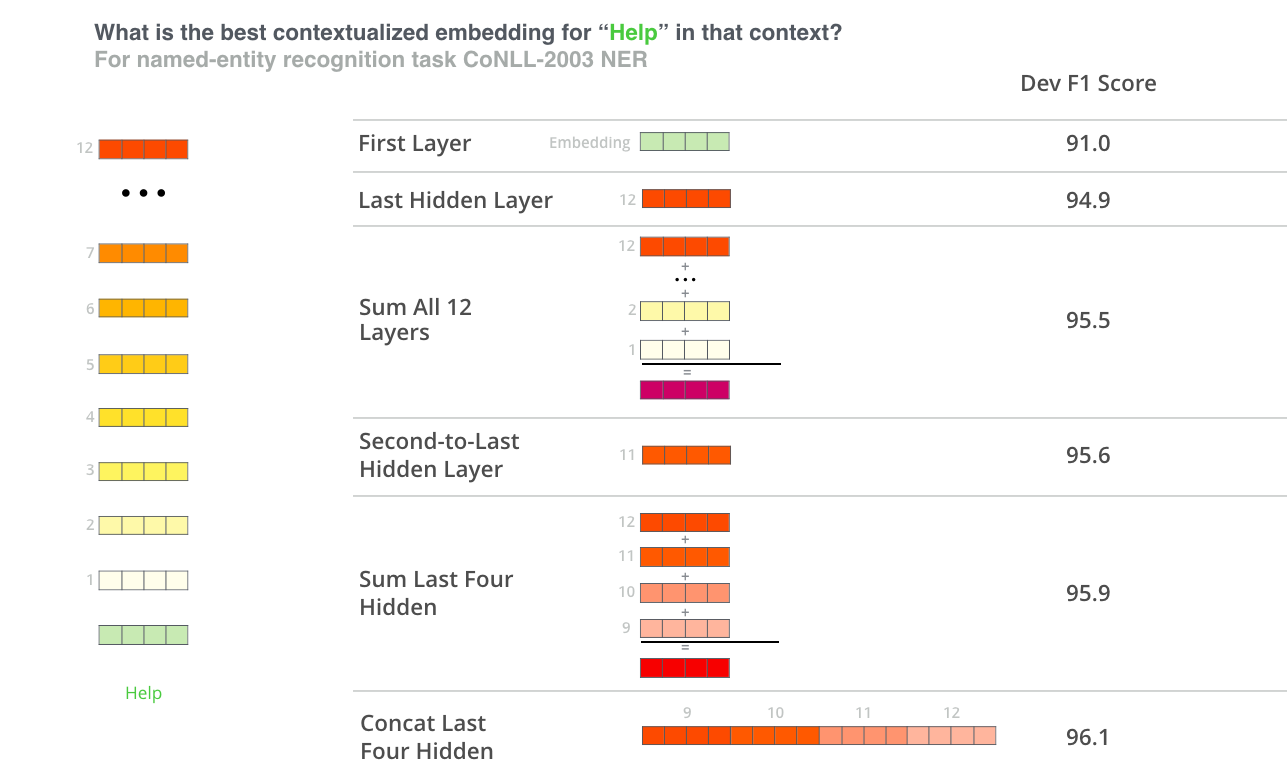
\includegraphics[width=0.6\linewidth]{image/irvrsv9mefroz7io6ilnjng3fo4}
	\caption{Возможные варианты получения векторного представления}
	\label{fig:dif_vars_get_v}
\end{figure}

Описанным ранее методом обрабатываются все подготовленные предложения.
В словаре модели BERT, представлены не все слова.
Слова, которых нет в словаре, модель разбивает на N-граммы символов.
Эмбеддинги получаются именно для N-грамм, некоторые слова делятся на N-граммы по 2 символа.
Данные векторные представления уже невозможно использовать для задачи пропорциональной аналогии, так как на этапе тестирования уже нельзя будет определить каким словам соответствуют эти N-граммы.

Есть 3 способа решить эту проблему.
Первый способ -- получить эмбеддинги для всех токенов, но на этапе тестирования брать только те пары слов, для который есть векторные представления.
В названиях моделей, использующих данный способ, не будет индексов.

Второй способ заключается в том, чтобы объединить N-граммы в первоначальное слово, а в качестве векторного представления посчитать величину среднего эмбеддинга для всех использованных токенов.
В названиях моделей, использующих данный способ, будет индекс \textit{2}.

Третий способ похож на второй, но с одним исключением.
Будет считаться не средняя величина эмбеддингов, а их сумма.
Данных подход похож на то, как с векторными представлениями N-граммов работают в модели FastText.
В названиях моделей, использующих данный способ, будет индекс \textit{3}.

Ожидается, что лучшее качество покажет первый способ, однако его тестовый датасет будет меньше, чем у второго и третьего способов. 

%Обработка происходит пачками по 10 тысяч предложений.
%Векторные представления токенов каждой пачки сохраняются на Google диск.
%Сделано это из-за ограничений оперативной памяти устройства.
После того, как получены векторные представления для всего текста, считаются средние эмбеддинги для каждого токена во всех контекстах.
Данные эмбеддинги уже готовы к тестированию.
%Из-за ограничений оперативной памяти нельзя посчитать сразу все векторные представления, поэтому они считаются порциями с сохранением промежуточных результатов.

\textit{ELMo.} Использовалась одна реализация модели ELMo, а именно модель в реализации от DeepPavlov.
Модель обучена на большом объеме данных из русской Википедии.
Порядок обработки текста аналогичен порядку обработки текста модели BERT, но с одним исключением.
В модели BERT был свой токенизатор, который обрабатывал входящие предложения.
Для ELMo такого инструмента нет, поэтому входящий текст необходимо токенизирвоать.
Из этого вытекает то, что слова не будут разбиваться на N-граммы и обработку N-грамм для ELMo можно будет пропустить.

ELMo создает векторные представления размерностью 1024, модели ELMo будут с припиской elmo.

В сумме получилось 14 моделей векторного представления слов.
Используется две модели BERT с тремя способами работы с N-граммами и одна модель ELMo.
При этом каждая модель будет работать на текстах двух жанров.

\begin{comment}
content...

\begin{enumerate}
	\itemsep0em
	\item bert-base-multilingual-cased-liter -- модель на основе bert-base-multilingual-cased, эмбеддинги получены на жанре литературы, функции обработки N-грамм не применялись;
	
	\itemsep0em
	\item bert-base-multilingual-cased-liter2 --  модель на основе bert-base-multilingual-cased, эмбеддинги получены на жанре литературы, в качестве эмбеддинга N-грамм брался их средний эмбеддинг;
	
	\itemsep0em
	\item bert-base-multilingual-cased-liter3 -- модель на основе bert-base-multilingual-cased, эмбеддинги получены на жанре литературы, в качестве эмбеддинга N-грамм бралась их сумма;
	
	\itemsep0em
	\item bert-base-multilingual-cased-polit -- модель на основе bert-base-multilingual-cased, эмбеддинги получены на жанре политики, функции обработки N-грамм не применялись;
	
	\itemsep0em
	\item bert-base-multilingual-cased-polit2 -- модель на основе bert-base-multilingual-cased, эмбеддинги получены на жанре политики, в качестве эмбеддинга N-грамм брался их средний эмбеддинг;
	
	
	\itemsep0em
	\item bert-base-multilingual-cased-polit3 -- модель на основе bert-base-multilingual-cased, эмбеддинги получены на жанре политики, в качестве эмбеддинга N-грамм бралась их сумма;
	
	\itemsep0em
	\item DeepPavlov-liter --  модель на основе DeepPavlov/rubert-base-cased-sentence, эмбеддинги получены на жанре литературы, функции обработки N-грамм не применялись;
	
	\itemsep0em
	\item DeepPavlov-liter\_2 -- модель на основе DeepPavlov/rubert-base-cased-sentence, эмбеддинги получены на жанре литературы, в качестве эмбеддинга N-грамм брался их средний эмбеддинг;
	
	\itemsep0em
	\item DeepPavlov-liter\_3 -- модель на основе DeepPavlov/rubert-base-cased-sentence, эмбеддинги получены на жанре литературы, в качестве эмбеддинга N-грамм бралась их сумма;
	
	\itemsep0em
	\item DeepPavlov-polit -- модель на основе DeepPavlov/rubert-base-cased-sentence, эмбеддинги получены на жанре политики, функции обработки N-грамм не применялись;
	
	\itemsep0em
	\item DeepPavlov-polit\_2 -- модель на основе DeepPavlov/rubert-base-cased-sentence, эмбеддинги получены на жанре политики, в качестве эмбеддинга N-грамм брался их средний эмбеддинг;
	
	\itemsep0em
	\item DeepPavlov-polit\_3 -- модель на основе bert-base-multilingual-cased, эмбеддинги получены на жанре политики, в качестве эмбеддинга N-грамм бралась их сумма;
	
	\itemsep0em
	\item elmo-DeepPavlov-liter -- 
	
	\itemsep0em
	\item elmo-DeepPavlov-polit -- 
\end{enumerate}
\end{comment}
	
\subsubsection{Визуализация данных}

Для наглядного представления эмбеддингов слов спроецируем их на плоскость.
Сделаем это при помощи метода понижения размерности, а именно метода главных компонент (PCA, principal component analysis).
Данный метод позволяет сохранить глобальную структуру данных, а также дает возможность проанализировать взаимное расположение слов.

\subsubsection{Оценка результатов}

Результаты будут получены для каждой модели, каждого жанра текста, для групп с разными связями между словами.
Будут проведены эксперименты с различными приемами работы с N-граммами.
Будет выяснено возможно ли аффинные преобразования в семантических пространствах контекстуализированных моделей и оценено их качество.

\subsubsection{Программная часть}

Для проведения экспериментов выбран язык программирования python.
Выбор языка программирования основан на том, что именно на python реализованы и обучены модели векторного представления слов.

В качестве IDE будет использоваться Jupyter Notebok от Google Colab.
Выбор Jupyter Notebok основан на том, что это удобный инструмент для аналитической работы, который позволяет интерактивно взаимодействовать с кодом.
Google Colab был выбран в качестве платформы для работы с Jupyter Notebok по следующим причинам:

\begin{enumerate}
	\itemsep0em 
	\item Предоставление мощных устройств c 12ГБ оперативной памяти с возможностью подключения GPU и TPU;
		\itemsep0em 
	\item Возможность запустить параллельно несколько Jupyter Notebok для увеличения скорости работы;
			\itemsep0em 
	\item Доступ к Google диску для чтения исходных данных и записи результатов.
\end{enumerate}

В качестве хранилища данных используется корпоративный Google диск так, как у него большая вместимость и есть возможность работать с Google Colab.
Для увеличения скорости обработки будем параллельно запускать несколько Jupyter Notebok в Google Colab.
В процессе обработки данных над одной моделью могут одновременно работать несколько устройств, но одно устройство работает только над одной моделью.

При обработке предложений их порядок не меняется и все предложения поделены на пронумерованные пачки по 1000 штук.
Во время обработки предложений устройство проверяет с какими номерами не хватает на диске пачек, если такие есть, то создается пустой файл с номером пачки, чтобы обозначить, что пачка с данным номером уже обрабатывается и другие устройства не начали работать над этими же данными.
после окончания обработки пачки результат также сохраняется с номером пачки.
По окончанию процесса все пустые файлы удаляются.

Алгоритм агрегации слов построен похожим образом.
Но перед началом необходимо составить словарь используемых слов и файлов, в которых эти слова хранятся.
Словарь также делится на пачки определенной длины и обрабатывается несколькими устройствами.
Важно перед началом агрегации скопировать все эмбеддинги на устройство, чтобы постоянно не гонять много данных через Google диск.
В противном случае можно получить бан от Google диска.

Далее остаются менее ресурсозатратные операции, которые в состоянии выполнить одно устройство.

В качестве фреймворков для работы с моделями векторного представления слов используются библиотеки transformer и tensorflow для BERT и ELMo соответственно.
Выбор данных фпеймворков основан на том, что у них есть доступ реализациям необходимых моделей векторного представления слов.

Ожидается, что объем эмбеддингов будет большим и оперативной памяти может не хватить, поэтому все данные будем обрабатывать пачками и сохранять на Google диске.
Хранить данные будем в бинарном формате pickle, данный формат позволяет хранить структуры данных python на диске без дополнительной обработки.

Для отрисовки графиков используется библиотека matplotlib.
Данная библиотека является мощным и удобным инструментом для работы с графиками.
Для подсчета косинусного расстояния используется функция cosine из библиотеки scipy.

Ссылки на репозиторий с кодом и на примеры получения и тестирования моделей находятся в приложении Б.
\newpage
\section{Практическая часть}

\subsection{Техническая часть}

Для работы модели BERT используется библиотека transformers, которая имеет реализации многих моделей машинного обучения, основанных на модели Transformer.
При обработке текста предложения подаются в модель по-одному, на выходе получается 4 мерный тензор, описанный ранее, типа torch.Tensor.
Полная обработка миллиона предложения для 1 модели на 1 устройстве занимает около 30 часов.
Для увеличения скорости обработки данных один и тот же текст обрабатывало сразу несколько устройств, при этом все данные отправлялись на один Google диск в формате pickle.
В зависимости от модели объем полученных эмбеддингов достигает 40 ГБ.

Для работы модели ELMO был использован tensorflow\_hub для скачивания модели и tensorflow версии 1.15, так как только для этой версии tensorflow есть русская версия ELMo.
На этапе тестирования была выявлена проблема того, что модель ELMo не оптимизирована под получение эмбеддингов слов в отдельных предложениях.
Из-за этого оперативной памяти устройства хватало для обработки 22-25 предложений и приходилось вручную перезапускать среду выполнения.
Это резко ограничило объем текста, обрабатываемого моделью ELMo.
Для модели ELMO обработано только по две тысячи предложений каждого жанра.
Полученные эмбеддинги также сохранялись в формате pickle на Google диск.

Далее обработка моделей BERT и ELMO совпадает.
Процесс агрегации эмбеддингов может достигать 20 часов при выполнении на 1 устройстве в зависимости от количества уникальных токенов.
Данный процесс также выполняется на нескольких устройствах с сохранением результатов на Google диск.

\subsection{Визуализация векторных представлений}

Визуализируем векторные представления при помощи метода главных компонент.

На рисунках \ref{fig:pril2}, \ref{fig:pril3} и \ref{fig:elmopil} изображены векторные представления для тестовых пар из группы <<прилагательное -- сравнительная степень>>.

\begin{figure}[H]
	\centering
	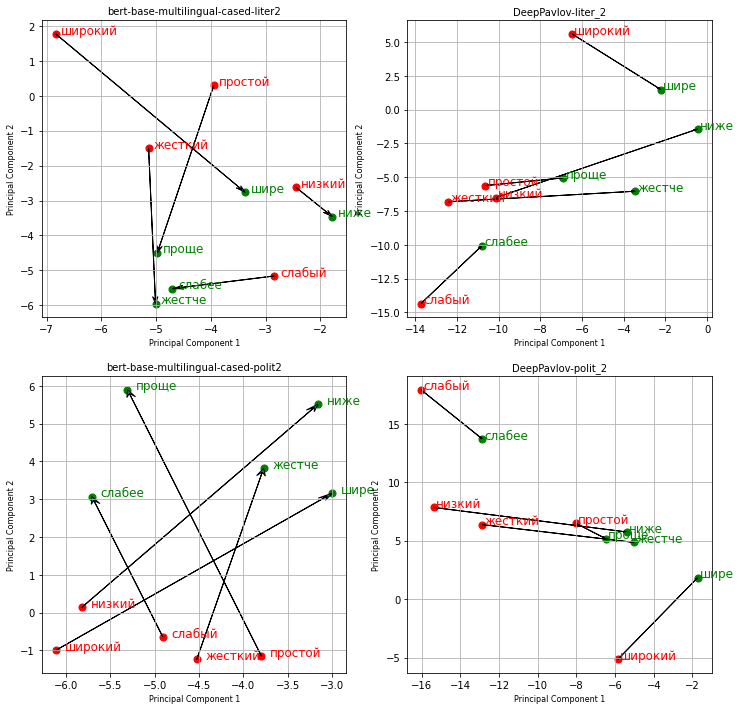
\includegraphics[width=0.5\linewidth]{image/pril_2}
	\caption{Визуализация эмбеддингов из группы <<прилагательное -- сравнительная степень>> для модели BERT с обработкой N-грамм через вычисление среднего эмбеддинга; Слева модель bert-base-multilingual-cased, справа от DeepPavlov; Верхние модели обучены на жанре литературы, нижние на политике}
	\label{fig:pril2}
\end{figure}

\begin{figure}[H]
	\centering
	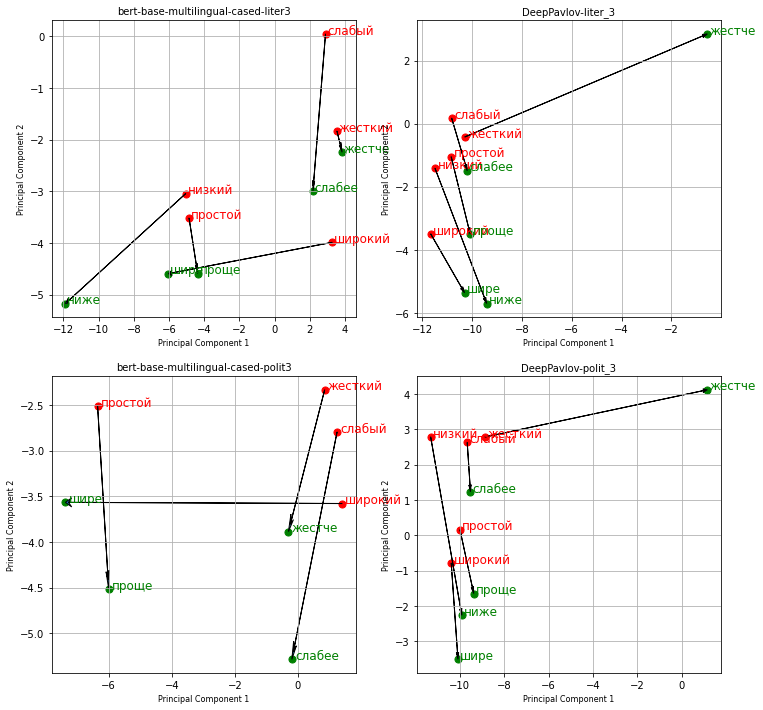
\includegraphics[width=0.5\linewidth]{image/pril_3}
	\caption{Визуализация эмбеддингов из группы <<прилагательное -- сравнительная степень>> для модели BERT с обработкой N-грамм через вычисление суммы эмбеддингов; Слева модель bert-base-multilingual-cased, справа от DeepPavlov; Верхние модели обучены на жанре литературы, нижние на политике}
	\label{fig:pril3}
\end{figure}

\begin{figure}[H]
	\centering
	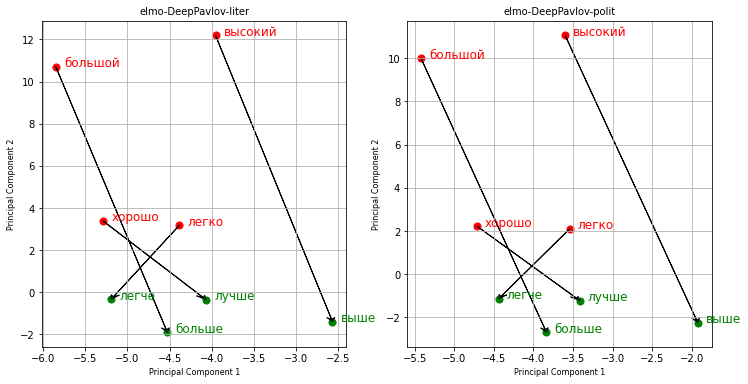
\includegraphics[width=0.5\linewidth]{image/elmo_pil}
	\caption{Визуализация эмбеддингов из группы <<прилагательное -- сравнительная степень>> для модели ELMo; Слева модель обучена на жанре литературы, справа на политике}
	\label{fig:elmopil}
\end{figure}

Первое слово в паре отображается красным цветов, второе -- зеленым.
Стрелки направлены от первого слова ко второму.
В приложении В находятся рисунки \ref{fig:pril2}, \ref{fig:pril3} и \ref{fig:elmopil} в лучшем качестве, а также визуализация группы <<мужской пол -- женский пол>>.
 
На первый взгляд, все вектора расположено хаотично, но в некоторых примерах прослеживается тенденция того, что вектора направлены в одну сторону.
В идеальном случае задачи пропорционального переноса вектора должны быть сонаправлены и быть равной длины.
По данным визуализациям можно предположить, что модели не смогут достичь идеального качества.

В визуализации векторных представлений модели ELMo (рисунок \ref{fig:elmopil}) можно заметить, что вектора разности при изменении жанра почти не изменяются.
Из этого можно сделать вывод, что в модели BERT контекст сильнее влияет на векторные представления, чем в модели ELMo.

Отобразим на плоскости векторные представления во всех контекстах (красные) и их среднее значение (зеленое) на плоскости.
На рисунке \ref{fig:moscow} векторные представления слова <<Москва>>.

Все точки можно условно поделить на 2 группы, справа и слева от центра, опытным путем было установлено, что группа справа отвечает за слова на кириллице, в группу слева входят слова, написанные на латинице. 

\begin{figure}[H]
	\centering
	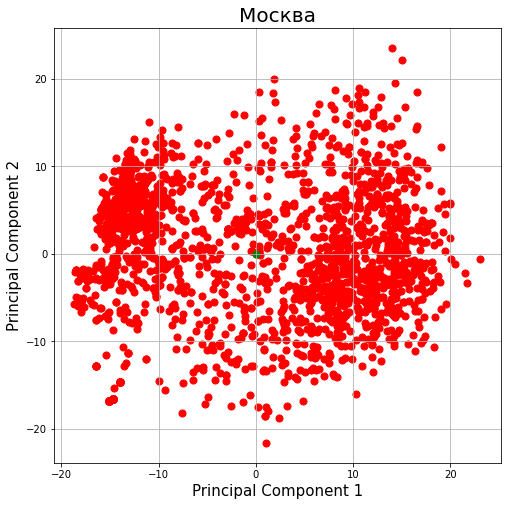
\includegraphics[width=0.5\linewidth]{image/moscow}
	\caption{Визуализация всех векторных представлений модели BERT для слова <<Москва>>}
	\label{fig:moscow}
\end{figure}


\subsection{Получение результатов тестирования}

На рисунках \ref{fig:resdeeppavlov-liter}, \ref{fig:resdeeppavlov-liter2}, \ref{fig:resdeeppavlov-liter3} и \ref{fig:reselmo-deeppavlov-liter} представлены результаты нескольких моделей.
Результаты тестирования всех моделей отображены в приложении Г.

Первая колонка описывает вид связи в группе.
Строка \textit{metric} указывает на использованный метод оценки.
Колонка \textit{accuracy} отражает долю верных ответов.
Колонка \textit{cosine} отображает среднее косинусное расстояние между посчитанным эмбеддингом и правильным эмбеддингом.
Последняя колонка описывает количество тестов в группе.

Не во всех таблицах с результатами присутствуют все 6 строк с тестируемыми группами.
Это произошло из-за ограниченности словарей моделей.
В случае с ELMo сильно сказался объем обрабатываемых текстов.

\begin{figure}[H]
	\centering
	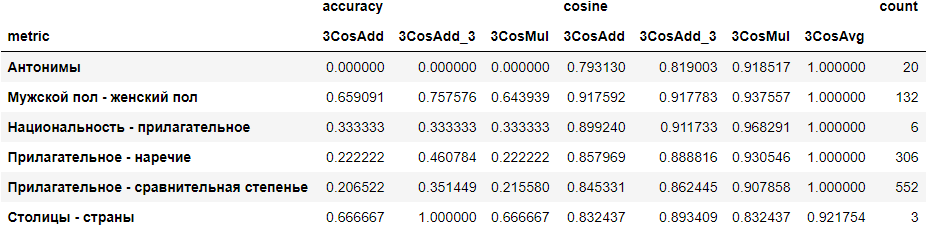
\includegraphics[width=0.8\linewidth]{image/res_DeepPavlov-liter}
	\caption{Результаты тестирования модели BERT от DeepPavlov без обработки N-грамм, обученной на жанре литературы}
	\label{fig:resdeeppavlov-liter}
\end{figure}
\begin{figure}[H]
	\centering
	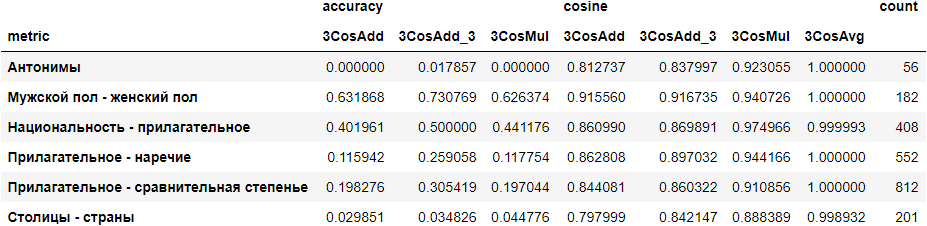
\includegraphics[width=0.8\linewidth]{image/res_DeepPavlov-liter_2}
	\caption{Результаты тестирования модели BERT от DeepPavlov с обработкой N-грамм через вычисление среднего эмбеддинга, обученной на жанре литературы}
	\label{fig:resdeeppavlov-liter2}
\end{figure}
\begin{figure}[H]
	\centering
	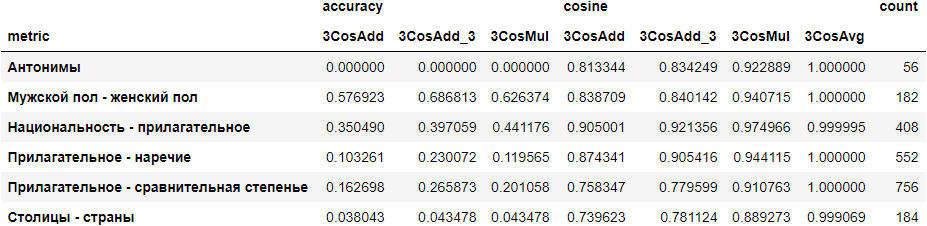
\includegraphics[width=0.8\linewidth]{image/res_DeepPavlov-liter_3}
	\caption{Результаты тестирования модели BERT от DeepPavlov с обработкой N-грамм через вычисление суммы эмбеддингов, обученной на жанре литературы}
	\label{fig:resdeeppavlov-liter3}
\end{figure}
\begin{figure}[H]
	\centering
	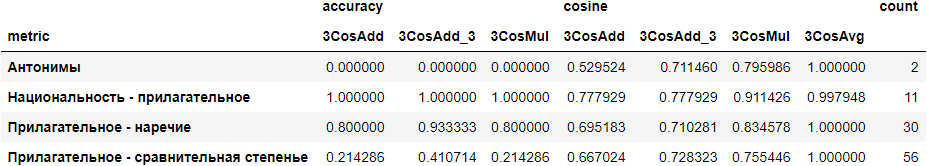
\includegraphics[width=0.8\linewidth]{image/res_elmo-DeepPavlov-liter}
	\caption{Результаты тестирования модели ELMo, обученной на жанре литературы}
	\label{fig:reselmo-deeppavlov-liter}
\end{figure}

Данные результаты показывают, что аффинные преобразования в модели BERT возможны, но их качество плохое.
Это может быть связано с тем, что в эмбеддингах помимо семантического смысла скрывается другая информация о словах, например, вектор позиционного кодирования.
При этом, качество аффинных преобразований модели ELMo на некоторых тестовых группах довольно высокое.

Результаты метода 3CosAvg показывают, что аффинные преобразования работают почти идеально.
Это можно объяснить тем, что модели неплохо распознают общий семантический смысл слов и в методе 3CosAvg от моделей не требуется четкий ответ в виде слова, им достаточно дать векторное представление.
Следует понимать, что в таблице округленные, хоть и до 6 знака после запятой.
%То же самое подтверждает и косинусное расстояние, целевой вектор и посчитанный вектор находятся близко друг к другу.

Результаты у методов 3CosAdd, 3CosAdd\_3 и 3CosMul получились невысокими из-за того, что рядом с целевым вектором находится много других векторных представлений, которые по смыслу близки к целевому слову.

Проведенные эксперименты показали, что задачу пропорциональной аналогии не всегда можно решить простым параллельным переносом.
Семантическое пространство имеет сложную структуру и нельзя с помощью простого параллельного переноса точно определить значение слова.
Несомненно, определенные закономерности в параллельном переносе присутствуют и можно приблизительно узнать значение полученного слова.
При помощи метода главных компонент было выявлено, что на векторное представление влияет множество факторов: архитектура модели, данные используемые для обучения модели векторного представления, данные используемые для получения эмббеддингов, методы работы с N-граммами и многие другие факторы.
Подытоживая, можно сказать, что для решения задачи пропорциональной аналогии параллельного переноса недостаточно, для ее решения необходимы более продвинутые методы преобразования векторов. 


%Еще одной из возможных причин плохого качества может быть то, что исследование проводилось на русском языке и не все слова из тестового датасета были в словаре модели BERT.

%
%\begin{enumerate}
%	\itemsep0em 
%	\item 
%\end{enumerate}

\newpage
\section{Заключение}

Модели векторного представления слов являются важной частью в автоматической обработке естественного языка.
В процессе обучения модели векторного представления слов ориентируются на контекст слова, при этом каждому слову сопоставляется вектор определенной размерности.
Данные векторы образуют семантическое векторное пространство.
В задаче пропорциональной аналогии предлагается выразить семантическую связь между парой слов в виде вектора разности, и утверждается, что для других пар слов с такой же семантической связью вектор разности векторных представлений будет совпадать.
Данный вопрос широко исследовался для различных неконтекстуализированных моделей таких, как word2vec или FastText, где эмбеддинги одного и того же слова в разных контекстах будут одинаковыми.
Но он не исследовался для контекстуализированных моделей таких, как BERT или ELMo.
В этих моделях векторное представление одного и того же слова в разных контекстах будет отличаться.
Это помогает модели лучше передать смысл слова в данном контексте.
Особенно это заметно на примерах омонимов.

В данной работе исследуются аффинные преобразования в семантических пространствах контекстуализированных моделей.
Был разработан метод для оценки параллельного переноса в этих моделях.
Были получены эмбеддинги слов на основании текстов двух жанров и трех моделей векторного представления.
Также был подготовлен датасет с раличными типами аналогий.
Были проведены численные эксперименты с использованием 4 методов оценки аффинных преобразований: 3CosAdd, 3CosAdd\_3,  3CosMul и 3CosAvg.
В ходе работы некоторые семантические связи были спроецированы на плоскость с использованием метода понижения размерности.

Численные эксперименты показали, что при решении задачи пропорциональной аналогии параллельный перенос не всегда дает верные ответы.
Семантическое пространство имеет сложную структуру и нельзя с помощью простого параллельного переноса точно определить значение слова.
При этом общий семантический смысл модель находит довольно неплохо.
Было установлено, что на векторное представление влияет множество факторов: архитектура модели, данные используемые для обучения модели векторного представления, данные используемые для получения эмббеддингов, методы работы с N-граммами и многие другие факторы.
Для решения задачи пропорциональной аналогии применение одного параллельного переноса мало, для решения этой задачи требуются более продвинутые методы работы с векторами. 

Данная работа может быть основой для последующих исследований контекстуализированных моделей векторного представления.
В качестве одного из направлений можно выделить кластеризацию эмбеддингов слов с целью поиска омонимов и определения их семантического значения.
Также можно выделить исследование семантической значимости одной или группы позиций в векторных представлениях слов.

\newpage 
\renewcommand{\refname}{{\normalsize \hfill Список использованных источников \hfill}} 
\bibliographystyle{unsrt}
\begin{thebibliography}{30}
	\addcontentsline{toc}{section}{Список использованных источников} 
% Введение
\bibitem{distrib}Harris Z. S. Distributional structure //Word. – 1954. – Т. 10. – №. 2-3. – С. 146-162.

\bibitem{w2v}Mikolov T. et al. Distributed representations of words and phrases and their compositionality //arXiv preprint arXiv:1310.4546. – 2013.
\bibitem{w2vkor}Корогодина  О. В. Исследование аффинных преобразований в семантическом пространстве Word2Vec // вкр. – Московский институт электроники и математики им. А.Н. Тихонова, 2020.

\bibitem{elmo1}Peters M. E. et al. Semi-supervised sequence tagging with bidirectional language models //arXiv preprint arXiv:1705.00108. – 2017.

\bibitem{elmo2}McCann B. et al. Learned in translation: Contextualized word vectors //arXiv preprint arXiv:1708.00107. – 2017.

\bibitem{elmo3}Peters M. E. et al. Deep contextualized word representations //arXiv preprint arXiv:1802.05365. – 2018.

\bibitem{bert1}Devlin J. et al. Bert: Pre-training of deep bidirectional transformers for language understanding //arXiv preprint arXiv:1810.04805. – 2018.

\bibitem{squad}Rajpurkar P. et al. Squad: 100,000+ questions for machine comprehension of text //arXiv preprint arXiv:1606.05250. – 2016.

\bibitem{attention}Vaswani A. et al. Attention is all you need //arXiv preprint arXiv:1706.03762. – 2017.

\bibitem{ft}Joulin A. et al. Bag of tricks for efficient text classification //arXiv preprint arXiv:1607.01759. – 2016.

\bibitem{lstm}Hochreiter S., Schmidhuber J. Long short-term memory //Neural computation. – 1997. – Т. 9. – №. 8. – С. 1735-1780.

\bibitem{semi}Dai A. M., Le Q. V. Semi-supervised sequence learning //arXiv preprint arXiv:1511.01432. – 2015.

\bibitem{ulmfit}Howard J., Ruder S. Universal language model fine-tuning for text classification //arXiv preprint arXiv:1801.06146. – 2018.

\bibitem{transformers}Radford A. et al. Improving language understanding by generative pre-training. – 2018.

\bibitem{21}Levy O., Goldberg Y. Linguistic Regularities in Sparse and Explicit Word 	Representations // Proceedings of the Eighteenth Conference on Computational Natural Language Learning, 2014. P.171-180

\bibitem{28}Drozd A., Gladkova A., Matsuoka S. Word Embeddings, Analogies, and Machine Learning: Beyond King-Man+Woman=Queen // Conference: Proceedings of COLING 2016, the 26th International Conference on Computational Linguistics: Technical Papers, 2016. 
P.3519–3530.

\bibitem{27}Linzen T. Issues in evaluating semantic spaces using word analogies // Proceedings of the 1st Workshop on Evaluating Vector-Space Representations for NLP, 2016. P. 13–18.

\bibitem{deep}Kuratov Y., Arkhipov M. Adaptation of deep bidirectional multilingual transformers for russian language //arXiv preprint arXiv:1905.07213. – 2019.


\end{thebibliography}

\begin{comment}

\newpage

%\addcontentsline{toc}{section}{Приложение А}

\begin{flushright}
	Приложение А
\end{flushright}


\begin{center}
	Пример визуализации функции позиционного кодирования
\end{center}


\begin{figure}[H]
	\centering
	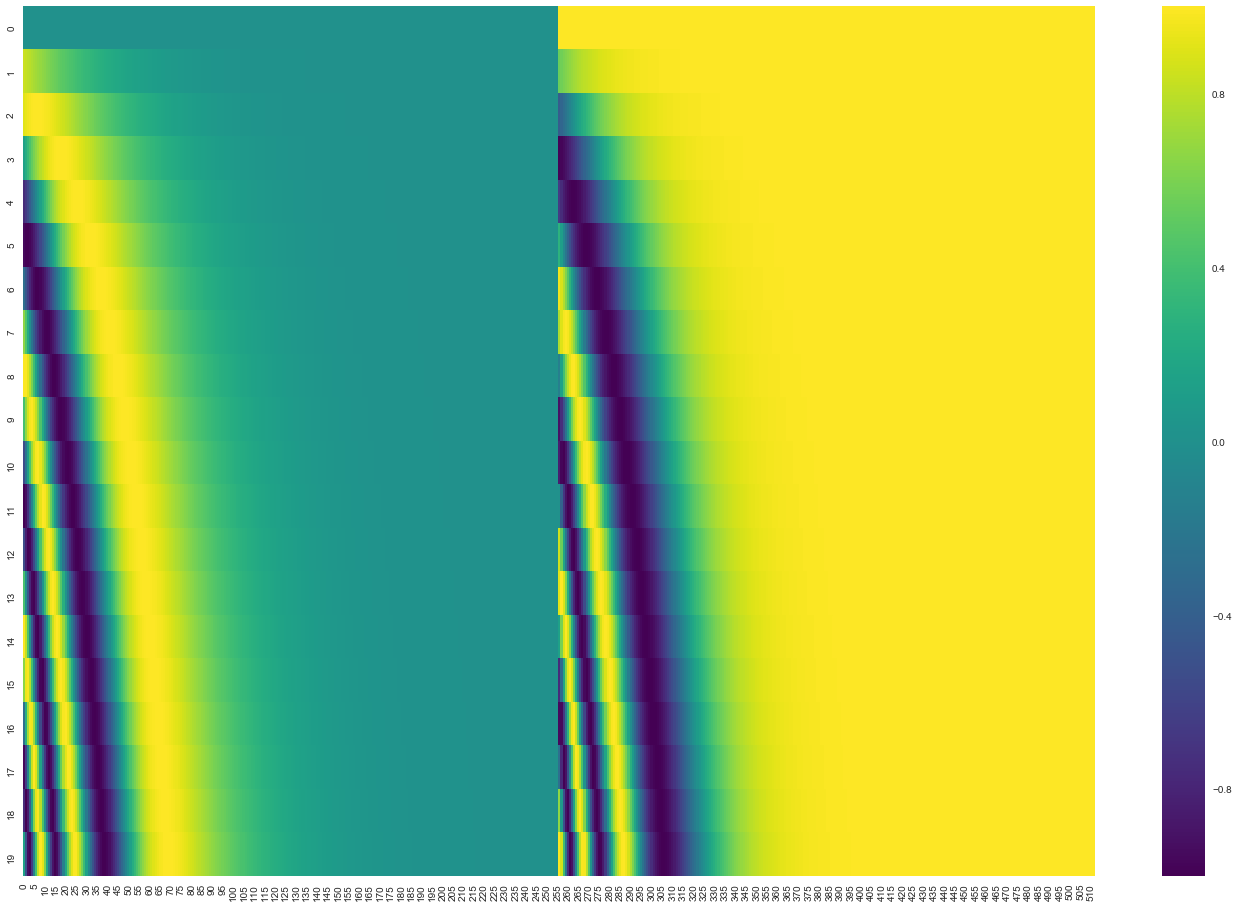
\includegraphics[width=0.95\linewidth]{image/v9dvohtljexbjop_vrykyyqdzbk}
	\caption*{Рис. А1. Пример визуализации функции позиционного кодирования}
	\label{fig:v9dvohtljexbjopvrykyyqdzbk}
\end{figure}

\newpage

%\addcontentsline{toc}{section}{Приложение Б}

\begin{flushright}
	Приложение Б
\end{flushright}

\begin{center}
	Визуализация эмбеддингов
\end{center}


\begin{figure}[H]
	\centering
	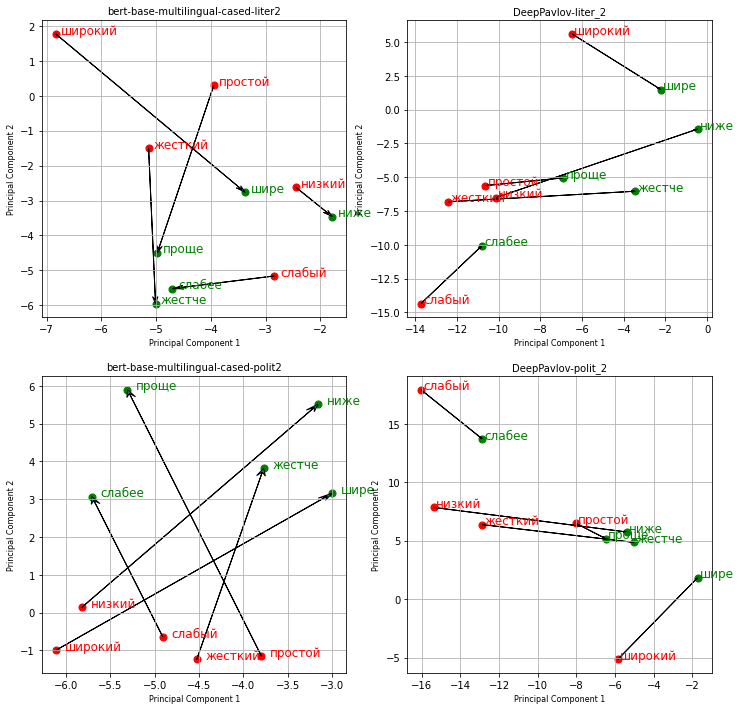
\includegraphics[width=0.95\linewidth]{image/pril_2}
	\caption*{Рис. Б1. Визуализация эмбеддингов из группы <<прилагательное -- сравнительная степень>> для модели BERT с обработкой N-грамм через вычисление среднего эмбеддинга; Слева модель bert-base-multilingual-cased, справа от DeepPavlov; Верхние модели обучены на жанре литературы, нижние на политике}
	\label{fig:pril22}
\end{figure}

\begin{figure}[H]
	\centering
	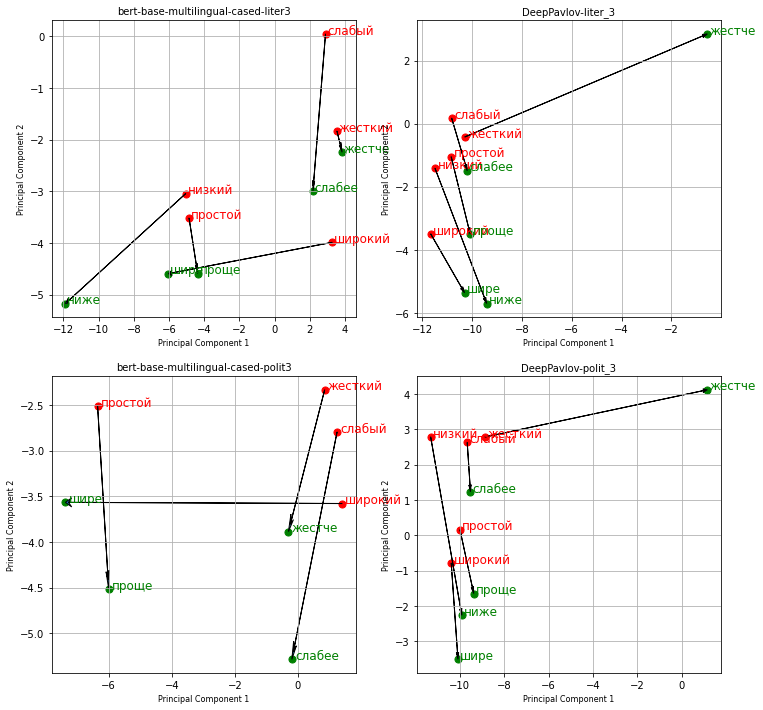
\includegraphics[width=0.95\linewidth]{image/pril_3}
	\caption*{Рис. Б2. Визуализация эмбеддингов из группы <<прилагательное -- сравнительная степень>> для модели BERT с обработкой N-грамм через вычисление суммы эмбеддингов; Слева модель bert-base-multilingual-cased, справа от DeepPavlov; Верхние модели обучены на жанре литературы, нижние на политике}
	\label{fig:pril32}
\end{figure}

\begin{figure}[H]
	\centering
	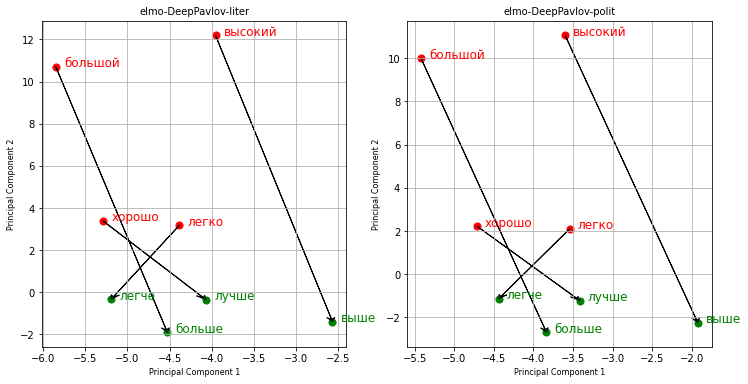
\includegraphics[width=0.95\linewidth]{image/elmo_pil}
	\caption*{Рис. Б3. Визуализация эмбеддингов из группы <<прилагательное -- сравнительная степень>> для модели ELMo; Слева модель обучена на жанре литературы, справа на политике}
	\label{fig:elmopil2}
\end{figure}

\begin{figure}[H]
	\centering
	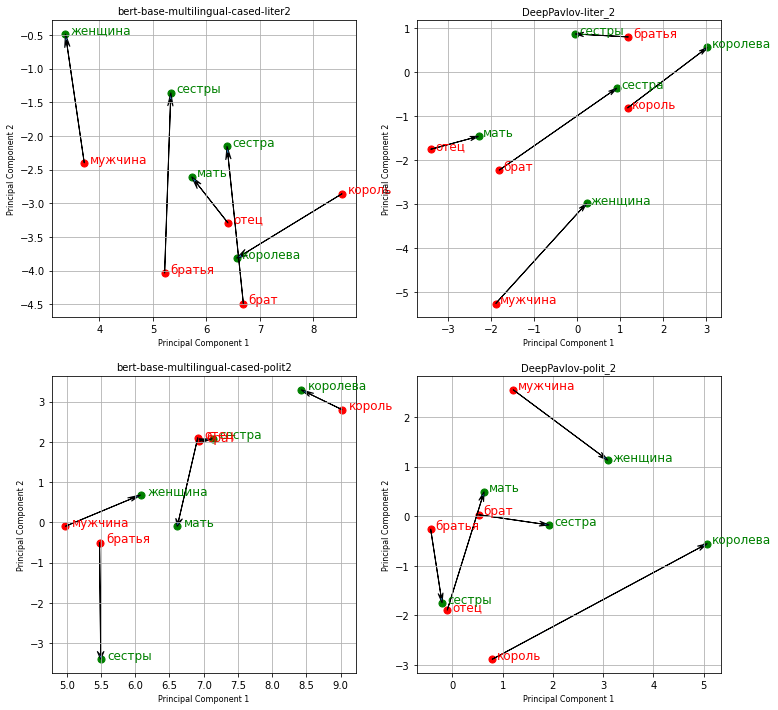
\includegraphics[width=0.95\linewidth]{image/fam_2}
	\caption*{Рис. Б4. Визуализация эмбеддингов из группы <<мужской пол -- женский пол>> для модели BERT с обработкой N-грамм через вычисление среднего эмбеддинга; Слева модель bert-base-multilingual-cased, справа от DeepPavlov; Верхние модели обучены на жанре литературы, нижние на политике}
	\label{fig:fam2}
\end{figure}

\begin{figure}[H]
	\centering
	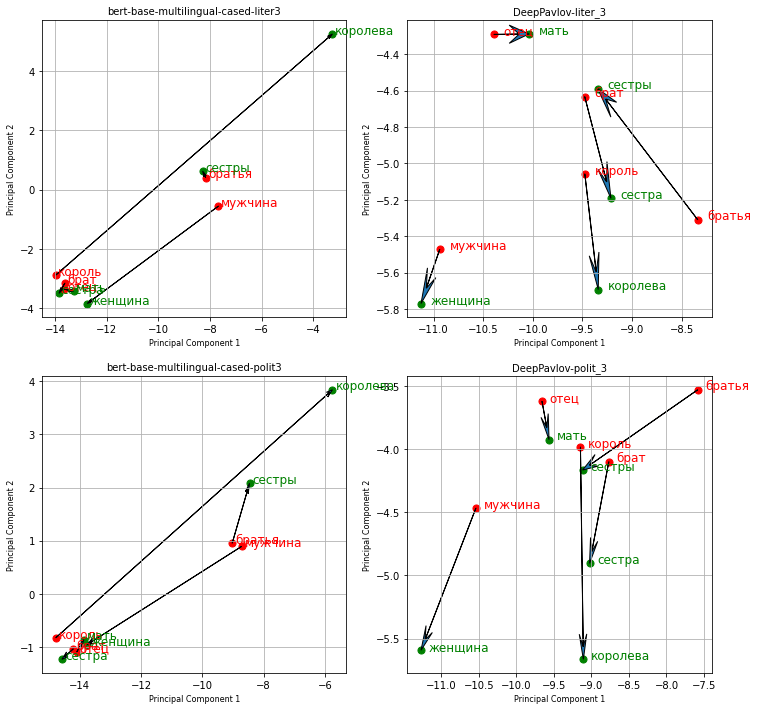
\includegraphics[width=0.95\linewidth]{image/fam_3}
	\caption*{Рис. Б5. Визуализация эмбеддингов из группы <<мужской пол -- женский пол>> для модели BERT с обработкой N-грамм через вычисление суммы эмбеддингов; Слева модель bert-base-multilingual-cased, справа от DeepPavlov; Верхние модели обучены на жанре литературы, нижние на политике}
	\label{fig:fam3}
\end{figure}

\newpage

%\addcontentsline{toc}{section}{Приложение B}

\begin{flushright}
	Приложение B
\end{flushright}

\begin{center}
	 Результаты тестирования моделей
\end{center}



\begin{figure}[H]
	\centering
	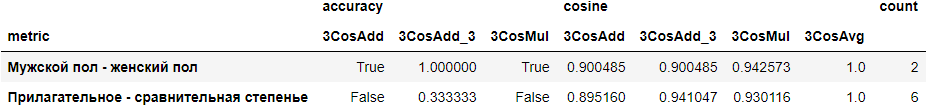
\includegraphics[width=0.9\linewidth]{image/res_bert-base-multilingual-cased-liter }
	\caption*{Рис. B1. Результаты тестирования для модели bert-base-multilingual-cased-liter }
	\label{fig:resbert-base-multilingual-cased-liter }
\end{figure}

\begin{figure}[H]
	\centering
	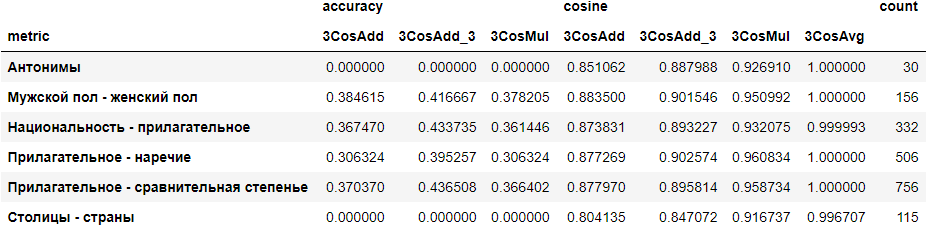
\includegraphics[width=0.9\linewidth]{image/res_bert-base-multilingual-cased-liter2 }
	\caption*{Рис. B2. Результаты тестирования для модели bert-base-multilingual-cased-liter2 }
	\label{fig:resbert-base-multilingual-cased-liter2 }
\end{figure}

\begin{figure}[H]
	\centering
	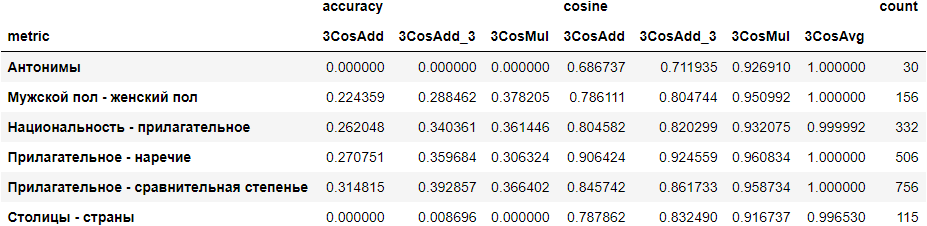
\includegraphics[width=0.9\linewidth]{image/res_bert-base-multilingual-cased-liter3 }
	\caption*{Рис. B3. Результаты тестирования для модели bert-base-multilingual-cased-liter3 }
	\label{fig:resbert-base-multilingual-cased-liter3 }
\end{figure}

\begin{figure}[H]
	\centering
	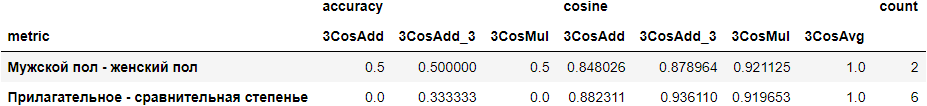
\includegraphics[width=0.9\linewidth]{image/res_bert-base-multilingual-cased-polit }
	\caption*{Рис. B4. Результаты тестирования для модели bert-base-multilingual-cased-polit }
	\label{fig:resbert-base-multilingual-cased-polit }
\end{figure}

\begin{figure}[H]
	\centering
	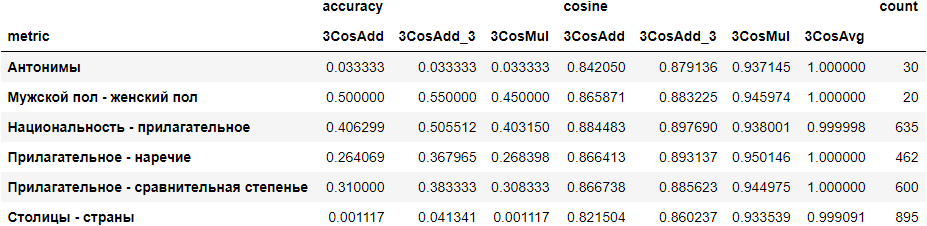
\includegraphics[width=0.9\linewidth]{image/res_bert-base-multilingual-cased-polit2 }
	\caption*{Рис. B5. Результаты тестирования для модели bert-base-multilingual-cased-polit2 }
	\label{fig:resbert-base-multilingual-cased-polit2 }
\end{figure}

\begin{figure}[H]
	\centering
	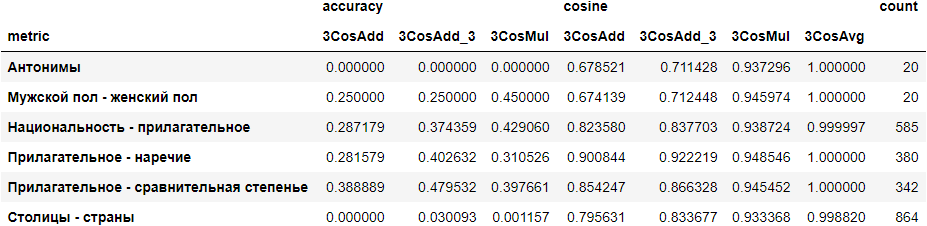
\includegraphics[width=0.9\linewidth]{image/res_bert-base-multilingual-cased-polit3 }
	\caption*{Рис. B6. Результаты тестирования для модели bert-base-multilingual-cased-polit3 }
	\label{fig:resbert-base-multilingual-cased-polit3 }
\end{figure}

\begin{figure}[H]
	\centering
	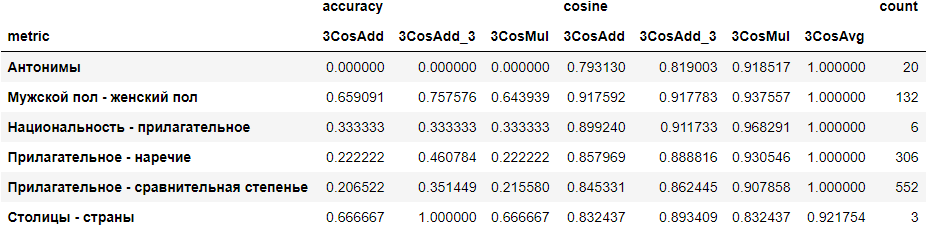
\includegraphics[width=0.9\linewidth]{image/res_DeepPavlov-liter }
	\caption*{Рис. B7. Результаты тестирования для модели DeepPavlov-liter }
	\label{fig:resDeepPavlov-liter }
\end{figure}

\begin{figure}[H]
	\centering
	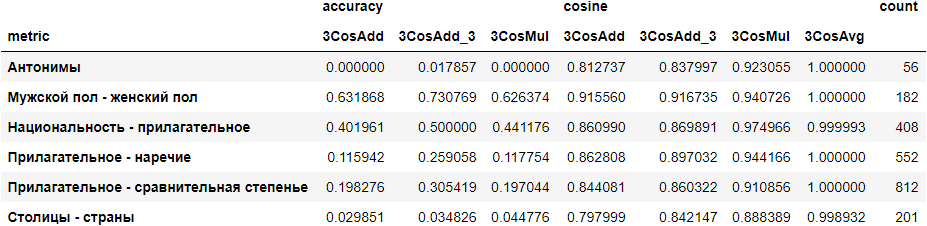
\includegraphics[width=0.9\linewidth]{image/res_DeepPavlov-liter_2 }
	\caption*{Рис. B8. Результаты тестирования для модели DeepPavlov-liter\_2 }
	\label{fig:resDeepPavlov-liter2 }
\end{figure}

\begin{figure}[H]
	\centering
	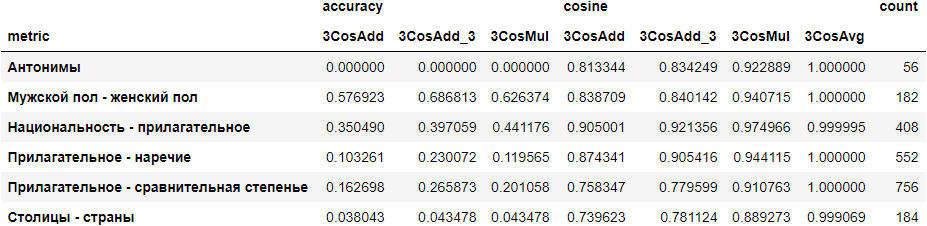
\includegraphics[width=0.9\linewidth]{image/res_DeepPavlov-liter_3 }
	\caption*{Рис. B9. Результаты тестирования для модели DeepPavlov-liter\_3 }
	\label{fig:resDeepPavlov-liter3 }
\end{figure}

\begin{figure}[H]
	\centering
	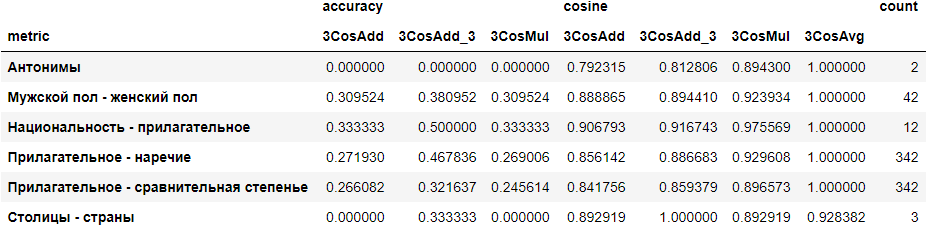
\includegraphics[width=0.9\linewidth]{image/res_DeepPavlov-polit }
	\caption*{Рис. B10. Результаты тестирования для модели DeepPavlov-polit }
	\label{fig:resDeepPavlov-polit }
\end{figure}

\begin{figure}[H]
	\centering
	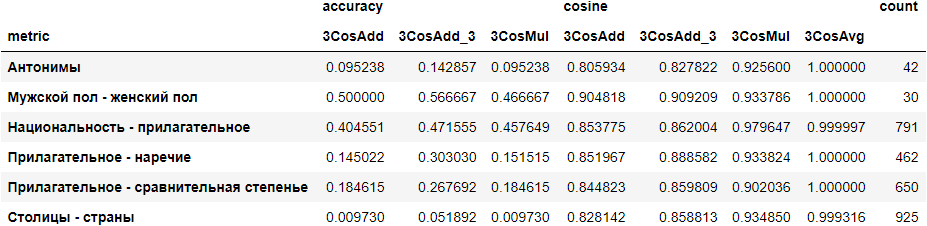
\includegraphics[width=0.9\linewidth]{image/res_DeepPavlov-polit_2 }
	\caption*{Рис. B11. Результаты тестирования для модели DeepPavlov-polit\_2 }
	\label{fig:resDeepPavlov-polit2 }
\end{figure}

\begin{figure}[H]
	\centering
	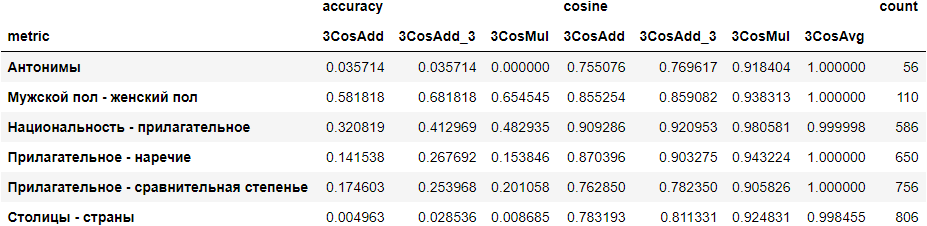
\includegraphics[width=0.9\linewidth]{image/res_DeepPavlov-polit_3 }
	\caption*{Рис. B12. Результаты тестирования для модели DeepPavlov-polit\_3 }
	\label{fig:resDeepPavlov-polit3 }
\end{figure}

\begin{figure}[H]
	\centering
	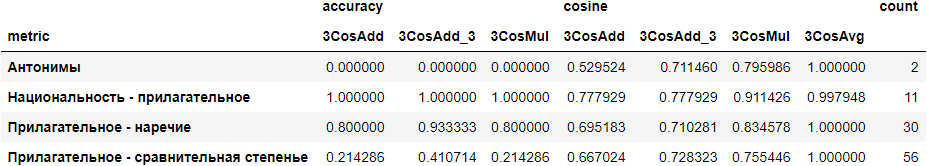
\includegraphics[width=0.9\linewidth]{image/res_elmo-DeepPavlov-liter }
	\caption*{Рис. B13. Результаты тестирования для модели elmo-DeepPavlov-liter }
	\label{fig:reselmo-DeepPavlov-liter }
\end{figure}

\begin{figure}[H]
	\centering
	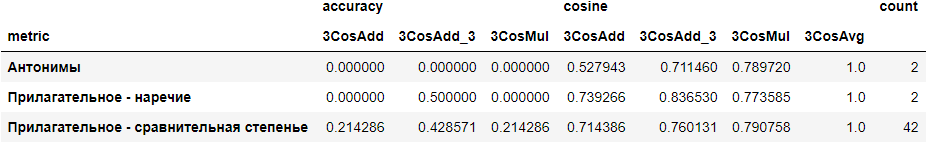
\includegraphics[width=0.9\linewidth]{image/res_elmo-DeepPavlov-polit }
	\caption*{Рис. B14. Результаты тестирования для модели elmo-DeepPavlov-polit }
	\label{fig:reselmo-DeepPavlov-polit }
\end{figure}

\newpage

%\addcontentsline{toc}{section}{Приложение Г}

\begin{flushright}
	Приложение Г
\end{flushright}

\begin{center}
	Ссылки на исходные коды
\end{center}

Ссылка на github репозиторий \href{https://github.com/andrsolo21/hse_Af_Tr_BERT}{https://github.com/andrsolo21/hse\_Af\_Tr\_BERT}.

Ссылка на ноутбук с примером работы модели BERT: \href{https://github.com/andrsolo21/hse_Af_Tr_BERT/blob/main/new_hse_BERT_0.ipynb}{https://github.com/andrsolo21/hse\_Af\_Tr\_BERT/blob/main/new\_hse\_BERT\_0.ipynb}.

Ссылка на ноутбук с примером работы модели ELMo:  \href{https://github.com/andrsolo21/hse_Af_Tr_BERT/blob/main/new_hse_ELMO_0.ipynb}{https://github.com/andrsolo21/hse\_Af\_Tr\_BERT/blob/main/new\_hse\_ELMO\_0.ipynb}.

Ссылка на ноутбук с агрегацией результатов: \href{https://github.com/andrsolo21/hse_Af_Tr_BERT/blob/main/Visualization.ipynb}{https://github.com/andrsolo21/hse\_Af\_Tr\_BERT/blob/main/Visualization.ipynb}.
\end{comment}
\end{document}